\chapter*{Critical Language for Software}

The name of the architect Christopher Alexander is perhaps better known in programming
circles than among architects, so he makes for the perfect opening of a text that aims
to find new links between the world of architecture and the world of software. But let
me be clear that I reference Alexander mainly to highlight a question that he posed about
the software practice, rather than to draw inspiration for better software design from his
work, a task already done by others.\endnote{patterns, RPG, Steenson}

The question I want to refer to was raied by Alexander in a keynote that he delivered in
1996 at the annual ACM Conference on Object-Oriented Programs, Systems, Languages and
Applications (OOPSLA). This was not an incidental invitation. By the mid-1990s, Alexander's ideas
on pattern languages and design patterns were already influential in the computer science and
software engineering circles and many of those involved in bringing Alexander's ideas into the
world of software were regular participants at OOPSLA.

In his keynote, Alexander talked about his lifelong quest for creating living structures
in the world, i.e., beautiful structures where each element is in harmony with each other,
structures that evolve well and reflect natural inclinations of their human inhabitants.
In the last part of his talk, Alexander called upon the attendees to take responsibility
for the built environment and tackle the problem of generating living structures.
As Alexander pointed out, the idea of generative process is natural to computer scientists
and so they are well equipped for the task.

Alexander commented on a perceived ``undercurrent of unease as to where all
this---software design---is going''. In a ``very direct and blunt'' comment, he suggests that:

\begin{quote}
It could be thought that the technical way in which you [computer scientists] currently look at
programming is almost as if you were willing to be ``guns for hire.'' In other words, you are the
technicians. You know how to make the programs work. ``Tell us what to do daddy, and we'll do it.''
That is the worm in the apple.
\end{quote}
% https://www.patternlanguage.com/archive/ieee.html

One could conclude that computer scientists and programmers share their predicament with architects
who, as argued by Charles Jencks\endnote{p26} ``have little power, [and] are not in any better
position to command what is built.'' Perhaps like architects, computer scientists and programmers
being ``fairly low in the chain of command and needing jobs, are prone to compromise with the
state and the establishment.''

There may be some truth in that, but I believe this is not the entire truth. On a more basic level,
programming, computer science and software development lack the critical language that is needed
for thinking about the problem. In other words, regardless of whether we have the power to command
what is built, we do not know how to effectively critically question what is built, how to imagine
alternatives, and how to ironically poke at the undesirable characteristics of what is being built.

%\section{Critical Language for Software}
This text is an attempt to develop such critical language of software. To do so, I will draw on
a number of architects and architectural critics. Their work provides an inspiration for
what, I believe, is needed for software. Some of those critiques are in the form of written text,
but more notably, architects also use building plans and buildings themselves to raise important
points about architecture. I believe we, programmers and computer scientists, similarly need to
find ways of designing software that not only fulfils a certain function, but also raises critical
questions. I acknowledge a certain irony in my effort. What you are looking at is itself text
and not a piece of software.

Although I started with Alexander's comment and I share his belief that programmers and computer
scientists should not accept the role of ``guns for hire,'' my thinking follows a different
route than that suggested by Alexander---one that would likely not make Christopher Alexander
himself very happy.\endnote{Alexander Eisenmann debate \url{https://arahovsepyan.com/eisenmanalexander}}
Rather than seeking a way of building that achieves a living structure, I turn to debates
on architecture that emerged from post-modern critical architecture and debates about it.

Even if our sole goal as programmers and computer scientists was to produce ``living
structures'' in the world, I do not think we can achieve this without first having a critical
language that lets us reflect on our work, criticise existing approaches, deconstruct our creations
and look for alternative arrangements.

In other words, I believe there is a value in exploring disharmony\endnote{Agreeing with Eisenmann
in the debate} and in using a critical language of architecture---or in my case of software---to
criticise the state of the discipline and imagine new ways of thinking and new ways in which
software can support social structures. Although I mainly look to writing on post-modern ar
chitecture for sources of inspiration, the idea of using buildings to question established order
is by no means new. We can trace similar ideas to the rise of modernism in Europe following
the First World War when some architects ``overwhelemed by the nightmare of industrialization
(...) briefly speculate on alternative condition'':\endnote{Oppositions -- p52, p55}

\begin{quote}
It is not the crazy caprice of a poet that glass architecture will bring a new culture.
It is a fact. (\ldots) Therefore the European is right when he fears that glass architecture
might become uncomfortable. Certainly it will be so. And that is not its least advantage.
For first of all the European must be wrenched out of his coziness.
\end{quote}

On the next couple of pages, I will look at two themes from post-modern architecture that
highlight some of the aspects of the critical language developed by architects that I hope
to create for software. I will then return to methodological problem of how such language
can be structured.

%\newpage

\begin{figure}[t]
\vspace{-1em}
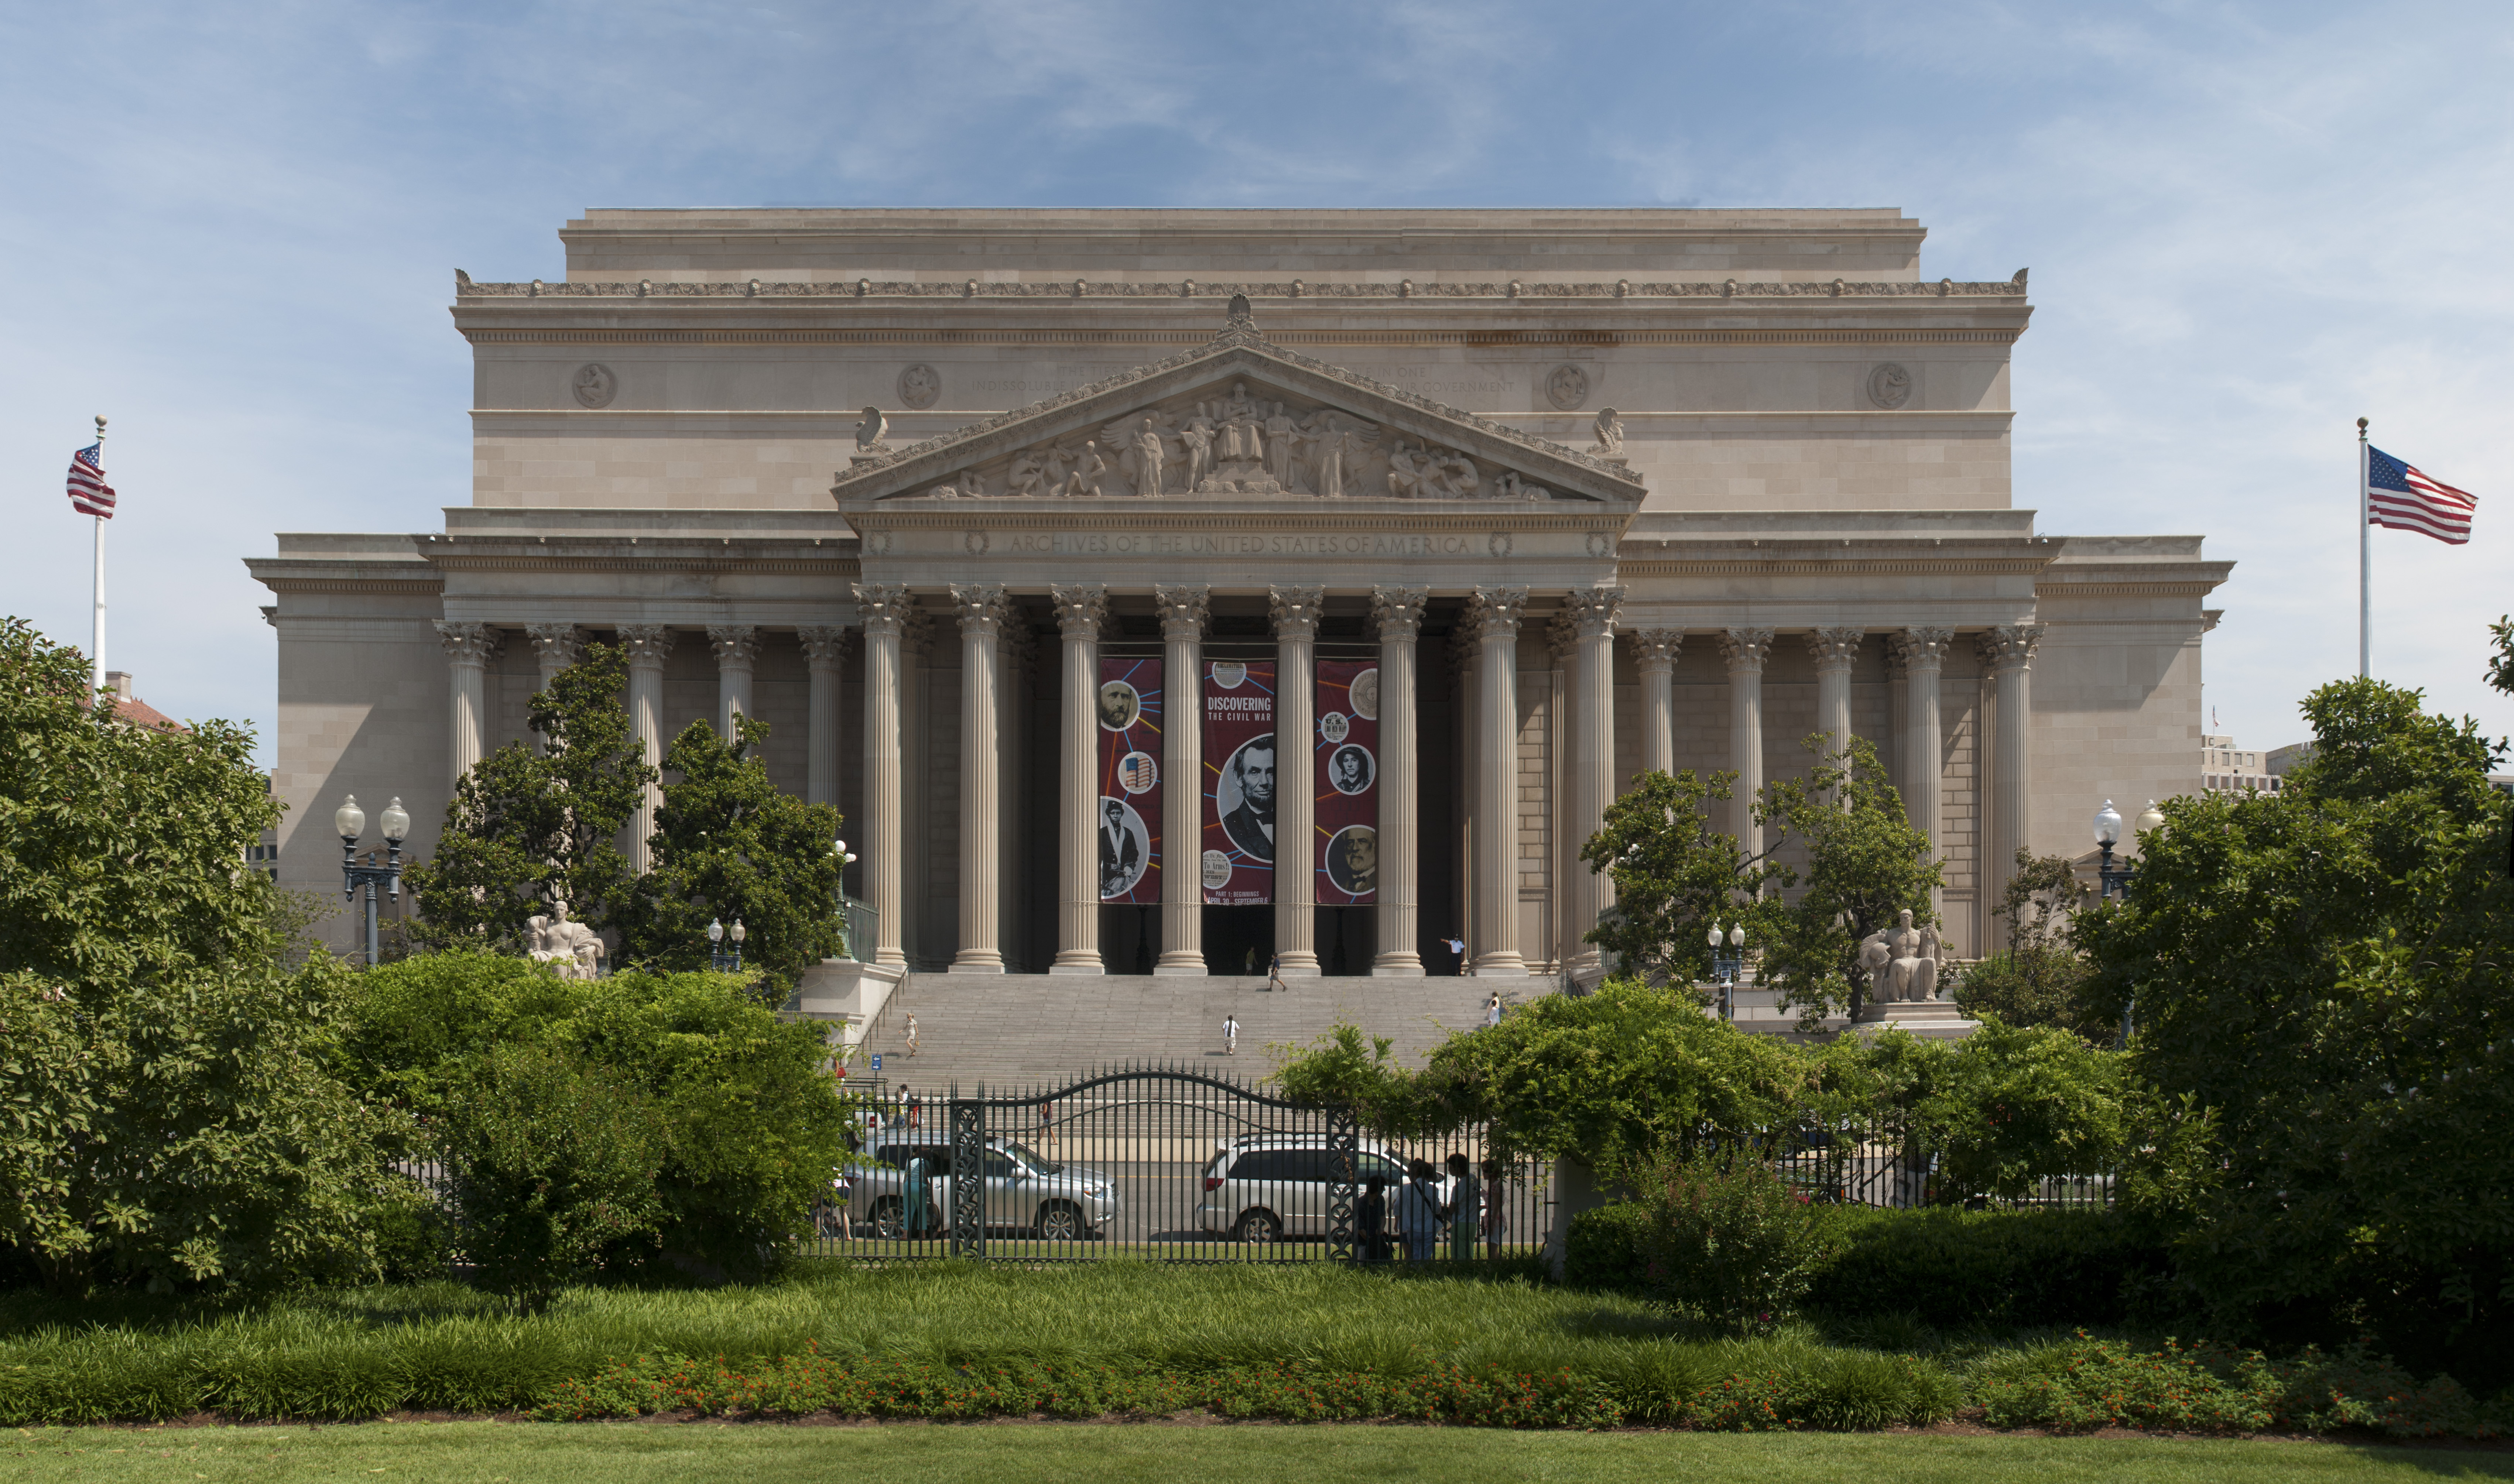
\includegraphics[height=9.85em]{fig/columns-archives.jpg}\quad
\includegraphics[height=9.85em]{fig/columns-savoye.jpg}\quad\\[1em]
\includegraphics[height=12em]{fig/columns-greek.jpg}\quad
\includegraphics[height=12em]{fig/columns-loos.png}\quad
\includegraphics[height=12em]{fig/columns-venice.png}\quad
\includegraphics[height=12em]{fig/columns-venturi.jpg}
\caption{Six different uses of columns in architecture. (1) Unironical use of the column in the 1935
neoclassical building of the US National Archives, (2) Supporting pilotis in Le Corbusiers 1931
Villa Savoye, (3) The Parthenon in Athens built in the 5th century BC according to the Doric order
(4) Adolf Loos' playful reference to the Doric column in a 1922 entry for the Chicago Tribune
Tower Competition, (5) Hans Hollein's ironical Facade of Morphed Columns, at the 1980 Venice
Architecture Biennale, and (6) Robert Venturi's ``ironic'' column from the 1977 addition to the
Allen Memorial Art Museum.}
\label{fig:columns}
\vspace{-1em}
\end{figure}

\section{The Ironical Column}
To illustrate some of the ways through which architects use architecture to communicate, I start
with the most basic structural element of classical architecture, the column. Figure~\ref{fig:columns}
shows several uses of columns, starting from the ancient Parthenon built in Athens in 5th century
BC (bottom left) followed by four examples that include a variety of references to the classical
column.\endnote{Idea from Oppositions p377, See also Korman ``The Architecture of the Facade'' -
for more on columns}

\newpage

Neoclassical architecture, which gradually grew in prominence in the late 18th century, looks
back to the Classical past. It sees it as a source of pure geometric order with ideal proportions
and symmetry. Such references to the ancients should not be unexpected. At the start of the 17th
century, Aristotle and other ancient philosophers were seen as the source of truth that was partly
lost and needs to be recovered, but that was already fully known to the ancients.\endnote{Wootton}
The scientific revolution of the 17th century gradually changed perspective on the ancients in what
was becoming experimental science, but it should not be a surpirse that architects of the 18th century
were still looking back to ancient structures that were becoming rediscovered and better understood
at the time. Neoclassical architecture remained influential after the 18th century, but its meaning
slowly shifted. It turned from an attempt to rediscover and recreate simple, purely geometrical
structures to an idealized style that emphasises tradition. The use of the style for many US federal
buildings is thus a reference to the values that the style encompasses.\endnote{Also conservative
``Executive Order on Promoting Beautiful Federal Civic Architecture'' -- Trump's administration (2020)}

The modernist Villa Savoye designed by Le Corbusier also looks back to the Classical past,
but it does so in a different way. Rather than directly copying the style and order of the
ancient Greek temples, the building is a reinterpretation of the ideas of a Greek
temple.\endnote{Unwin - Twenty-Five Buildings Every Architect Should Understand}
It reimagines the ideal structure of Greek temple based on geometric principles (using the golden
ratio), but replaces ancient Greek columns with minimalistic modernist pilotis. Following the
modernist focus on function, Le Corbusier's design uses pilotis to give prominence to the
automobile (parked on the ground floor). Although the same historical reference is present in Villa
Savoye, it is used at a more conceptual level and is not immediately apparent.

The importance of the column as an icon representing a certain style of architecture was well
understood by other modernist architects, including Adolf Loos who is best known as the author
of the modernist manifesto ``Ornament and Crime'', first presented as a lecture in 1910. In his entry
for the Chicago Tribune headquarters competition in 1922, Loos made yet another reference to the
ancient Greek temple and shaped the entire building as a giant Doric column.  Loos himself did not
view the column in his design as ornamental and instead saw it as supporting the public nature of
the building with appropriate symbolism.\endnote{Krul - Adolf Loos and the Doric Order}
The structure of the building itself here becomes the symbol in a way that is reminiscent
of later post-modernist works where construction patterns and material textures themselves become
ornament.\endnote{Jencks, p183} Despite being rooted in the modernist thinking, the Chicago Tribune
Tower project became an inspiration for later post-modern architects who make, more or less subtle,
historical references in an ironic way. They will include columns in their buildings to indicate
that they recognize being a part of architectural culture and tradition, even if they no longer
need columns as structural support mechanisms.

A good illustration of the ironic reference is the facade created by Hans Hollein for the 1980
Venice Biennale. The event took place in Corderia of the Arsenale, a large historical building
itself featuring supporting columns. The participants of the Biennale were asked to design a
facade for their exhibition that would cover (and hide) the historical structure of the Corderia.
Hollein did the exact opposite. He complemented two columns of the Corderia with a range of
ironical forms of columns. One was a bushy tree cut into the shape of a column, while another was
a scaled-down version of Loos' Chicago Tribune Tower. The entrance into the exhibition was under
a hanging fragment of a column, which clearly lost its original structural function, but gained
a different function as an exhibition entrance. Here, the ironical use of the architectural
language is direct and understandable.\endnote{Branscombe - Hans Hollein and Postmodernism}

Hollein's entry addressed the theme of the Biennale, ``The Presence of the Past'' in a way that
is funny and ironic, but sends a clear message about history and continuity of architecture. It
also illustrates the changing function of a column from supporting structure to a decoration. Moreover,
the ironical style of the presentation, shared with many other post-modern architectural works, makes
the message accessible and engaging for broader public. Hollein's facade is interesting for
yet another reason. It uses architectural language to communicate architectural ideas, but it
is neither text, nor a building. As we will see repeatedly, built structures such as stage sets
or monuments are often interesting media through which critical architectural ideas can be
expressed.

The column takes yet another form in the addition to the Allen Memorial Art Museum designed by
Robert Venturi in 1977. The extension itself is based on an idea that Venturi refers to as
the ``decorated shed''. The basic structure and spatial disposition of the building itself is
simple and serves its function which was, in part, to provide more storage space.
Any symbolic, cultural and aesthetic meaning is provided ``by modifying the basic shell by means
of design decisions of a second order.''\endnote{Oppositions, p182} One such second-order
decision is the addition of isolated iconic elements, such as the mock Ionic column that
marks the building as cultural institution. In a way, the column serves similar role as the
neoclassical architecture of the US National Archives, but is here added merely as an ironic
decoration. The association of ancient Greek columns with important public buildings remains,
but the story is told in a very different way.

% ~
%
% ~
%
% "Classicist tropes estranged from traditional use" - Aureli
%
%
% ironic historical reference - critical of neoclassicism
% change of function, repurpose
% exhibition - stage set / pavilions, allows for communication
% reveal inherent conflicts
% ironically distort regularity - point out things
% change of function - non-structural (decorated shed)
% irony valued for superior depth, allows showing multiple contradictory views (Jencks, 79)
% intellectual reference to other works vs. funny reference for broader public - to engage with wider audience!

\section{Towards Critical Software}

In my attempt to translate the critical langauge of architecture into the world of software,
I will alternate between two modes of working. First, I will reinterpret existing practices
in software development and computer science in light of the architectural theory. Second,
I will suggest how we could more deliberately follow in the footsteps of architects and
create new software artifacts that express critical points about software.

In other words, can we follow post-modern architects and embed criticism as a first-class
element in software practice, rather than leaving it to a second-class (and largely optional)
critical writing?\endnote{Oppositions 377, also Venturi introduction} We can also look to
post-modern architects for initial ideas of what such critical software can say. The
architectural style known as eclecticism makes funny references such as Hans Hollein who
decorated his Austrian Travel Agency office with metalic palm trees and broken Greek
column.\endnote{Jencks, p56} The appeal of the style is not just its straightforward humour,
but the fact that it is understandable and can communicate with wider audience. Similarly,
post-modern architects have used contextualism to highlight important characteristics of the
environment they work in or use references to suggest alternative social organization.

Looking at existing software practices, we can imagine how the above arhictectural ideas
can apply to basic structural elements from which software is built. One such element may
be the data structures around which software is structured.\endnote{ref Abstracting craft p96;
ref Joel - the other part of the basic structure is how change is described} Data structures
in software are arguably even more fundamental than columns in architecture, because any
software that works with data needs to store the data in some way. The limitation of this
metaphor is that, unlike columns which are typically visible, data structures are typically
hidden from the end-user. There also is no singular classical model of data structures,
although a number of models fit a similar role. These include the relational model of databases,
flat memory model of low-level programming languages and data types that model data as collections
of nested records.\endnote{Memory models blog}

We can use the architectural metaphor to talk about the differnt kinds of classical models
of data structures. Whereas the relatively expressive language of the relational model or
the nested records model could be linked to different kinds of classical columns, the minimalistic
models of flat memory or nested lists of the Lisp programming language are more akin to
modernists undecorated and purely functional pilotis.

When the data structures are used to store data, they serve the original intended purpose,
just like columns functioning as supporting structure. But equally, there are software systems
where data structures are used more as rhetorical elements, intended not for the computer
execution of the software, but for the end-user or programmer. One example would be types
in the TypeScript programming language. Here, the actual representation of data can be anything
permitted by the underlying JavaScript runtime. TypeScript type declarations are mere labels,
intended for the human and for the static TypeScript type checker, but they are not enforced or
used for checking at runtime. The type declarations still look like a definition of the shape
of a data structure (a column), but they no longer play the basic structural function. They are
used for paratial checking (a scaffolding around a column?) and as information for the
programmer (a purely rhetorical column). A similar case would be the use of data structures
in non-relational databases such as key-value stores or document databases. The data stored
in such systems in practice has some implicit structure.  However, any explicit description
of the structure is merely literal. The description may use the language of standard data
structures (collections, records, primitive types), but this is not used for representation.

Do certain data structures also have particular symbolic associations, in a manner similar
to how the Classical column stands for traditional values, often associated with US federal
buildings? I believe this is the case. For instance, the class-based object-oriented
programming paradigm is often associated with maintainability. Languages that adopt
class-based object-oriented abstractions as their basic data structure do not do so
just for practical, but also for symbolical reasons. TypeScript serves to illustrate this
again. One of the first books on the language claims that ``TypeScript [brings] a level of
maintainable structure to JavaScript development through its class and module
features.''\endnote{Dan Maharry, TypeScript Revealed, 2013} Written in the same year when
the language was released, the claim could not rely on empirical experience with the language,
but mainly on the symbolic associations of the data structure.

\begin{figure}
\begin{lstlisting}[language=csxml]
<CsamlFile xmlns="http://schemas.microsoft.com/winfx/2006/xaml/csaml"
      xmlns:x="http://schemas.microsoft.com/winfx/2006/xaml">
  <NamespaceDeclaration Identifier="MyNamespace">
    <ClassDeclaration Identifier="MyClass" Access="Public">
      <MethodDeclaration Identifier="Main" Access="Public"
            Modifier="Static" ReturnType="{x:Type void}">
        <InvocationExpression MemberAccess="System.Console.WriteLine">
          <InvocationExpression.ArgumentList>
            <Literal Type="{x:Type string}" Value="Hello, CSAML!">
          </InvocationExpression.ArgumentList>
        </InvocationExpression>
      </MethodDeclaration>
    </ClassDeclaration>
  </NamespaceDeclaration>
</CsamlFile>
\end{lstlisting}
\caption{The ``Hello world'' program written using the C\# Application Markup Language (CSAML),
conceived by Charles Petzold in an April Fool's post on 1 April 2006.}
\label{fig:csaml}
\end{figure}

For my last example based on a reference to an existing artefact, I want to show that
data structures have already been used to make critical ironical statements. The April Fool's
post written by Charles Petzold in 2006 introducing the ``C\# Application Markup Language''
is a illustration.\endnote{\url{http://www.charlespetzold.com/etc/CSAML.html}}
The post introduces a new notation that encodes programs written in the C\# language
using XML (Figure~\ref{fig:csaml}). The post can be seen as an ironical work of contextualism.
The post was published in the heyday of the XML format when Microsoft released multiple
development frameworks built around XML. As a well-written April Fool's joke, the post
made readers think. The post praises the semantic clarity of the XML format and gives
various examples that are extremely lengthy and tedious. After a brief puzzlement, most readers
realise the joke. But the post makes them wonder about the verbosity and unnecessary
overuse of the format at the time.

\begin{figure}
\centering
\includegraphics[width=0.75\textwidth]{fig/strip.jpg}\quad
\caption{``Exodus, or the Voluntary Prisoners of Architecture: The Strip (Aerial Perspective)''
by Rem Koolhaas, Elia Zenghelis, Madelon Vriesendorp and Zoe Zenghelis. The project
imagines a walled city of ``new urban culture'' within the city of London.}
% https://www.moma.org/collection/works/104692
\label{fig:exodus}
\end{figure}

The C\# Application Markup Language example hints at a number of themes that I will further
explore later. It is perhaps blatantly funny, but it can still be seen as making a serious point.
Moreover, the system that the post describes has never been actually implemented. The post
is merely a (very basic) plan for a system. This does not, however, make it any less valuable
as critical software. Many interesting pieces of critical architecture have also not been
built, yet, they became important references. The Chicago Tribune tower by Adolf Loos is one
such case, but even better example would be one of the many architectural projects that
use the architectural language to intentionally propose structures that cannot be built.
One such project is The Strip (Figure~\ref{fig:exodus}) by Rem Koolhaas. The project imagines
an enclosed restricted city cutting through London. Although the work was inspired by the
situation of West Berlin during the Cold War, the ideas of building a wall to separate cultures
can be seen in new (and alarming) light today.

In the subsequent chapters, we will see that hypothetical design proposals, fictional
plans that cannot be built or impractical systems are a powerful way of making a point
about software systems, just like they are a powerful way of making a point about architecture.
The C\# Application Markup Language can be seen an example of a much broader class of
esoteric programming languages, which are created jokingly, but can be often read as
valuable critiques.\endnote{Cox, Speaking Code}

\begin{figure}
\centering
\includegraphics[width=0.85\textwidth]{fig/pompidou.jpg}\quad
\caption{The Centre Pompidou ``inside-out'' building, which keeps all the infrastructure
(using green for plumbing, yellow for electricity, blue for climate control, and red for
circulation) on the outside to allow flexible and efficient use of the inside space.}
% https://www.flickr.com/photos/jeanbaptistem/5448056975/in/photolist-HFZ9L-k5DdGP-9iqHwP-4vkacq-ydwXxD-9K2Jaz-k5LueV-k5Lh5K-HFYXU-ySUqb4-k5MyjB-ebvgdy-ydouoL-k5CwUF-9K2J1z-k5CV3R-2o6FcFX-m7tSj-aAbT1J-23edLxs-f9M6TH-k5CR2x-k5BJ4g-k5Cz5K-98pso6-4H9NcH-k5Q4fu-QMA3dr-4HdZ6y-aSKucT-4H9Nii-4HdYXd-6NgNR9-aSKC7P-74qk4S-4EvW6x-4fdBW2-9K2NKp-ebpE8F-z9o7SU-7yeN5y-byStES-a9DTqd-2qvg1Dn-ecAeV-nU1orA-bMM8zr-4EAaLQ-k5KdY6-4beX5c
\label{fig:pompidou}
\end{figure}

As I wrote earlier, I believe that we can take inspiration from the critical architectural
language both to analyze existing software systems and projects, but also to come up with
new ideas. Some of the references to a column that I discussed earlier make points that
may well be applicable to software systems. For example, they may ironically highlight the fact
that a column is used for its symbolic value, but not for its original purpose.
They highlight the fact that it is no longer needed functionally, even if it is often used
for rhetorical reasons.
We can imagine a range of similar critical points to be raised about the technical concept
of data structures in the context of programming and software systems. If a column is no longer
needed as a structural element, what may be the established essential aspect of data structures
that is no longer needed?

One of the most established ideas associated with structuring application data is that of
information hiding.\endnote{Parnas, On the criteria; also reflections in \url{https://link.springer.com/chapter/10.1007/978-3-642-59412-0_25}}
The argument is that one should separate software systems into components that have a stable
public interface and private implementation. If one identifies suitable stable public interface,
it is possible to develop the components in isolation, change the implementation or replace
individual components as needed. But information hiding has also been criticised.\endnote{GPII Nexus,
my article on architecture, Convivial Design Heuristics for Software Systems} The problem is
that predicting what part of the interface should be fixed and what can be hidden is often
difficult, especially in the context of software systems whose function evolves and changes
over time. Clark and Basman\endnote{GPII nexus} quote the example of MIDI SysEx messages that
have, by convention, become a mechanism that exposes the state and can control the operation
of musical devices. This enabled MIDI to become a powerful music control platform in a way
that could not have been anticipated by the designers of the MIDI interface in the 1980s.
Arguably, an even more prominent example would be the web platform, where much of the data
structures that the web is built around (HTML, CSS) are also transparent.\endnote{But this
has limits, see my talk.}

So far, most ciritiques of information hiding have taken the form of text. To make the point
through the critical language of software, we should design an exemplar piece of software
or programming system that reverses the idea of information hiding. In other words, we
should expose all the underlying data structures of the software in a way that is akin to how
the Centre Pompidou (Figure~\ref{fig:pompidou}) exposes all the service infrastructure of the
building.

In such hypothetical system,\endnote{suggested by Clark and Basman} all the state of the system
would be externalised in a way that allows anyone to see and modify it. To make the point,
the system should do this to the extent possible. The accessible state should include all
information about the data structures, as well as execution of the system. Depending on the
chosen programming paradigm, this may include data of all objects, memory, stack, currently
executing instructions etc. The information should also be exposed in a way that makes it
available not just to the programmer,\endnote{this is already possible via reflection or in
image-based systems} but also to the end-user. The system would have to handle the fact that
its state may be modified in inconsistent ways and could either recover as best as possible
(akin to how web browsers recover when encountering invalid HTML) or break (likely making an
interesting point about the fragility of software systems).\endnote{c.f. antifragile}
The color coding used in the Centre Pompidou offers another interesting idea. If we exposed
all data structures of a software system using similar color coding (for different aspects
of the system), the system would increase public awareness about what modern software consists
of. Thus the project can also fulfil an educational function.

There is, of course, a practical issue of the context in which such project can become
reality. It is entirely possible to develop a critical software system only in the form of
specification or description, much like Charles Petzold's C\# Application Markup Language.
However, to explore the consequences of the design---and see how a system can be used in
the absence of information hiding---an actual non-trivial working implementation is needed.
I will return to this problem later, but architecture has a variety of options. Many
architects explore their theories for houses built for their own use or their
family.\endnote{Gehry's residence, Vanna Venturi house} Similarly, programmers and computer
scientists often have their own projects to experiment on.

Architecture also often speaks through
non-building objects such as stage sets, public monuments, pavilions and follies or exhibitions.
Those may not (yet) have obvious equivalents in the world of software and the task of developing
critical language of software may involve finding those. Last but not least, new architecture
also sometimes emerges in isolated places within a large city, called heterotopias in reference
to Michel Foucault.\endnote{Jencks, 119} Such isolated spaces, such as prisons, ghettos,
amusement parks, or leftover spaces known as terrain vague.\endnote{vagni teren}
I believe we can similarly find a range of atypical pieces of software, which are often deemed
as unimportant, but provide space for experimentation. Ad-hoc scripts, demos, spreadsheets,
and programs created at hackathons or coding competitions are only a few examples of hterotopias
in the world of software.

% Oppositions p376
%
% "criticism embedded in practice" (Venturi) - not just code, but also docs
% Eclecticism - be funny (Jencsk) - engage with audience in a fun way?
% Morality / social relevance (Jencks) - c.f. thimbl
%
% self-referential sign
% -> thing ported from (native) environment to expensiove recreation in another? (to keep UX or something?)
%
% serious artists engage with history, choosing what to keep and what to drop (The Hub)
% rebuilding old things anew?
% -> reconstructions
%
% Class as a column?
% basic structure, associated with maintainability...
% (evolved from closures and back)
%
% god object / class? - chicago tribune
%
% types and data structures - in cases where they are not enforced (nosql) - mere nice annotations
% - data structure characerizes software - Craft, p96
% => vocabulary for what you can do - disrupt? nosql databases (allow anything) -
% c.f. craft p98 (disrupt the gap in definining vs. understanding SW structures?)
%
% point out things that we're doing without thinking (information hiding)
% -> expose structure
%
% Rhetorical element? (Venturi)
%
% highlight contradictions - plenty in software
% hard to read architecture is valid if it reflects contradictions (Venturi)
%
% exhibitions / stage sets
% -> format for communication
% -> heterotopias (Jencks)
%
%
% Deconstruction
% - use some methodological way rigorously to show where it leads

\begin{figure}[t]
\vspace{-1em}
\includegraphics[height=8.5em]{fig/grammar-fascio.jpg}\quad
\raisebox{1.2em}{\boxed{\includegraphics[height=7em]{fig/grammar-formal.png}}}\\[1em]
\includegraphics[height=9.5em]{fig/grammar-house-x-model.jpg}\quad
\includegraphics[height=9.5em]{fig/grammar-house-x-diagram.jpg}\quad
\includegraphics[height=9.5em]{fig/grammar-la-vilette.jpg}\\[1em]
\includegraphics[height=11.1em]{fig/grammar-familian.jpg}\quad
\includegraphics[height=11.1em]{fig/grammar-memorial.jpg}
% fascio - wikipedia
% memorial - (cropped) https://www.flickr.com/photos/kevingessner/3323686050/in/photolist-64GL4U-gmYANP-6YkWHE-8vUy7Q-9FH37x-pVsPse-5d4N58-2dVZT3p-67BAtZ-or2tXp-84DzeG-84AtzF-LtDWre-5rERP4-AWVNRW-2nV1U1m-CJngd7-5UyjuF-d1g2U-64GLH7-8bsffq-6YQqX6-gmXTZg-641dZT-2p9SPMP-61vkjE-64GLx5-64GLm7-8L4PSH-CJnfyb-qzFxwu-qZ3YXX-edtnMV-bsDTdV-8mgDe1-MsMXg8-7h3Fnw-8L4PZr-gmYrDQ-6ekCEq-ni4YuS-djLNZH-8L4Q6z-CXjdR-CJu3nH-74y5Mo-FshXT-D8opnP-2p4e5P-nhKtYg
% familian - https://www.moma.org/collection/works/1020 (cropped)
% la vilette - https://eisenmanarchitects.com/La-Villette-1987
\caption{Five different uses of what can be interpreted as a formal language in architecture.
(1)~Modernist Casa del Fascio in Como, Italy built in 1936 and (2) a formal analysis of the building
by Peter Eisenman, (3) model of the House X, also by Eisenman and (4) a diagram illustrating
its formal structure based on the L-shape, (5) model from a 1987 project for a garden in the
Parc de la Villette by Eisenman in collaboration with Jacques Derrida, (6) model of the unbuilt
Familian Residence house by Frank Gehry from 1978, and (7) the Memorial to the Murdered Jews of
Europe designed by Eisenman, completed in 2004.}
\label{fig:grammar}
\vspace{-0.5em}
\end{figure}

\section{Formal Grammars of Architecture}

In the previous two sections, I focused on ideas that approach architecture from
the particular, specifically the structural element of a column. I will now look at ways
of developing critical language for architecture starting from the general.
I look at a number of works, most notably by Peter Eisenman, that relate architecture to
language, art and their formal structures and grammars (Figure~\ref{fig:grammar}).

The most direct reference to formal grammar in the context of architecture comes
from Peter Eisenman's PhD thesis, completed in 1963 at University of Cambridge. His thesis,
``The Formal Basis of Modern Architecture'' is concerned with formal analysis of
form and formal order in modern architecture. Eisenman suggests that the architectural form
can be seen as a problem of logical consistency, rooted solely in the properties of basic
structures from which the architectural form arises. The view opposed that of modernists who saw
form as arising from function, as well as Christopher Alexander's view put forward in his
Notes on the Synthesis of Form.\endnote{see debate} In contrast with modernists:

\begin{quote}
Eisenmann saw modernist forms not as simple derivatives of functional needs, but as
delineations of the immanent self-referntial properties of architectrue itself,
as searches for objective knowledge that lies outside both the architural agent's intentions
and the building's uses, and inside the very materials and formal operations of
architecture.\endnote{Oppositions, x}
\end{quote}

The time was probably right for this kind of intellectual project.
Eisenman was influenced by his reading of the linguist Noam Chomsky,\endnote{Oppositions, 202}
who published his first work on formal languages and grammars at the end of the 1950s. The
same ideas also contributed to the development of formal grammars of programming languages at
the end of the 1950s.\endnote{Algol}

Eisenman's thesis is analytical. He considers the plans of a range of modern buildings,
including those by Le Corbusier, Mies van der Rohe and Alvar Aalto, and explains their
structure in terms of a number of simple formal principles. Those include three basic
kinds of movement systems throughout the building (pinwheel, spiral, echelon), three types
of volumetric systems (horizontal planes, vertical planes, plaid) and various interactions
between them that lead to distortions of and dislocations in the basic structure.

One building analyzed by Eisenman is the modernist Casa del Fascio in Como designed by
Giuseppe Terragni. Eisenman sees the formal structure of the building as the product of
``reconciliation between a centroidal plan and a linear site.''\endnote{Formal basis, p293}
The form is a hollowed out cube. The cube can be seen as a series of planes, which needs
to be acknowledged by the side facades and which imposes a connection between the front and
the rear facade. To accommodate access to the inner courtyard, which results from the centroidal
plan, the ``negative volume is then dislocated'' giving the frontal facade reading of
an H-form.

Eisenman's analysis may seem like a curious theoretical exercise, but architects who study
the structure or the langauge of architecture had a more fundamental objective. Their aim
was to establish autonomous architecture, that is architecture that ``opens the internal
processes of architecture to their own internal possibilities.''\endnote{Autonomy and the Will to
the Critical - Eisenman} In other words, they seek architecture that is not created in response
to various external forces (of which there are many), but that is rooted in its own basic
(necessary) principles.

Eisenman himself went on to explore various uses of a formal architectural
grammar, not just analytically, but also as the basis for new designs in his numbered series of
houses, some built and some unbuilt. The House X, for instance, is a critique of ``the idea of
development from simple to complex''\endnote{Oppositions, p219} by using the L-shape as the
starting point, replacing the conventional cube. The design questions the humanist ideology
by disrupting the centrality that is typical of most houses. Where one might expect a hearth or
a staircase, there is nothing. The fact that this introduces a degree of disharmony in the project
has become contentious issue. While, Eisenman argued that an importnat role of art and architecture
is reminding people that ``everything isn't all right'', Christopher Alexander in a debate said
that such design makes him ``incredibly angry'' and he saw projects that introduce disharmony
as ``fucking up the world''.\endnote{debate}

In the 1980s, the experiments with architectural language, its grammar and the decomposition
of architectural structures took another form. Influenced by the French philosopher Jacques
Derrida, architects started to use architectural language to question the basic structures
and their conventional meaning. Eisenman himself collaborated with Derrida on a
project for a garden in the Parc de la Villette. The proposal eventually developed\endnote{Chora L
Works} into a scheme that rescales and overlays a number of different structures including
historical state of the site when it was a part of city walls and other projects by Eisenman
and his collaborators.

The almost mechanical design method is used to destabilize traditional
values of architecture such as its human scale and function. The authors propose to do this by
making parts of the park unexpectedly large or small, or by making parts inaccessible.
The La Villette project thus uses the architectural language to question the basic assumptions
of architecture. The project, again, causes the kind of disharmony that would enrage Christopher
Alexander.

In a critical commentary on the Parc de la Villette, Jeffrey Kipnis explained that
the point of deconstruction is to ``battle with the very meaning of architectural
meaning.''\endnote{Kipnis in Chora L works, p137} Because ``deconstruction deconstructs the
homogeneity, the unity of style`` it cannot, according to Jacques Derrida yield to
a single architectural style. Yet, this is what, perhaps somewhat inadvertently, happened
in the 1980s when the theoretical works of Eisenman got jointly exhibited with more literal
or pragmatic works by architects such as Frank Gehry, Zaha Hadid or the Austrian firm Coop
Himmelb(l)au.\endnote{Deconstruction in Architecture, at Tate and Deconstructivist Architecture
at MoMA, both 1988.} % https://www.dezeen.com/2022/05/20/deconstructivism-architectural-design-magazine-andreas-papadakis/

An early example of what became known as deconstructivist architecture is the series of Frank
Gehry's residential designs of the late 1970s and early 1980s. Gehry's work combines
experiments with different materials and spatial dynamics with the rejection of the modernist
grid.\endnote{See Frank Gehry, Architect: The Art of Architecture (Guggenheim Museum Publications)}
His formal structures are inspired less by grammars of Chomsky, but by avant-garde artists.
For example, the ``main masses [of his Familian Residence house] form a clearly Supermatists
grouping, recalling Malevich's Red Square and Black Square.''\endnote{The secret life of buildings:
An American mythology for modern architecture}
As noted by Charles Jencks, ``Gehry’s method of Deconstruction can be quite literal at
times, since he will smash an existing building into parts, leave elements of his own work
unfinished and (...) make an aesthetic virtue of rough, crumbled surfaces.''\endnote{Deconstruction
in Architecture (Papadakis, ed.) - p18} Yet, despite the different aesthetic and conceptualization
of the work, there is a clear connection between the work of Eisenman and Gehry. In some of their
works, they both try to uncover basic forms that comprise architectural structures and reveal them
through distortion.

The formal abstract structure, resulting from the composition of primitive architectural forms,
was also the basis for Eisenman's design for the Memorial to the Murdered Jews of Europe,
also known as the Holocaust Memorial in Berlin. The same formal mechanisms that were used as
a critique of humanism in architecture are used to create an unnerving experience for the
visitor.\endnote{Callaghan, M. (2020). Empathetic Memorials. Palgrave Macmillan Memory Studies.}
The abstract form of the memorial, devoid of symbolism and narrative, ``grants no further
understanding, since understanding the Holocaust is impossible.''\endnote{\url{https://eisenmanarchitects.com/Berlin-Memorial-to-the-Murdered-Jews-of-Europe-2005}}
In other words, the Holocaust Memorial is a structure that calls exactly for the kind of
disconcerting disharmony that Eisenman explored in his early house designs. According to
a brief explanation provided by Eisnman:\endnote{\url{https://eisenmanarchitects.com/Berlin-Memorial-to-the-Murdered-Jews-of-Europe-2005}}

\begin{quote}
This project manifests the instability inherent in what seems to be a system, here a
rational grid, and its potential for dissolution in time. It suggests that when a supposedly
rational and ordered system grows too large and out of proportion to its intended purpose,
it loses touch with human reason. It then begins to reveal the innate disturbances and potential
for chaos in all systems of apparent order.
\end{quote}

The formal architectural language explored by Eisenman since the start of his career thus
finds a new kind of use in the memorial. As with the Facade of Morphed Columns for the Venice
Biennale, the Holocaust Memorial is a different kind of architectural place, or a heterotopia,
where different architectural language can be, and needs to be, explored.

%
% circular houses, external storage; move to private rectangular houses with storage
% move to private houses (Aureli p88)
%

\begin{figure}
\centering
\vspace{-1em}
\includegraphics[width=0.65\textwidth]{fig/axonometric.jpg}\quad
\caption{Axonometric model of House X, which is a three-dimensional construction,
made to provide the image of a two-dimensional drawing from one particular angle.}
% https://eisenmanarchitects.com/House-X-1975
\label{fig:axonometric}
\end{figure}

\section{Questioning the Structure of Software}
Architects who probe formal structures of the architectural language may do so to better understand
the language, uncover assumptions that we accept and rarely question and explore consequences of
changing or manipulating the language. As in the previous section, this is often done using the
architectural language itself. Eisenman's numbered series of houses, Gehry's residences and Parc
de la Villette were all planned to be built and a number of them still stand.\endnote{And even houses
built to question the humanist focus of architecture sometimes found their satisfied owner.
\url{https://www.nytimes.com/2002/10/10/garden/house-proud-a-white-elephant-reincarnated.html}}
This fact, again, points at the possibility of a critical language that is not external to the subject
matter, but integrated within it. That is, the use of architecture to make critical architectural points
or, in the case I am interested in, the use of programming and software to make critical points about
software.

In some cases, architects use other formats too. Eisenman's doctoral work was a text presenting
a formal analysis of existing buildings. The deconstructivist practice can be used to probe the
process of architecture, as well as other artifacts it involves. For example,
Eisenman also criticises humanist ideology of architecture through the
axonometric model of the House~X (Figure~\ref{fig:axonometric}), which makes
``the `normal' image appear to be an anomaly.''\endnote{Oppositions, 219}
Similarly, computer scientists and programmers should include a broader range of materials in
their notion of critical language of software, including formal definitions, software
specifications and demonstrations. Those can, no doubt, be constructed in a similarly
illuminating distorted manner as Eisenman's axonometric model.

The analytical way of looking at basic structures of the language of the subject matter is something
that computer scientists are well familiar with. It has been done at multiple levels. On one
level, formal models of computations such as Turing machines and the lambda calculus have been
used to describe the basic structure of computation. Like the grammar that reduces architecture
to relationships between basic shapes, formal models of computation reduce program execution to
a minimal set of operations. That said, there is a difference between computing and architecture
in that formal models of computation originate in logic and have been conceived to study
computability properties, rather than originating in the analysis of existing programs.

\begin{figure}
\centering
\includegraphics[width=0.7\textwidth,trim=0cm 13.5cm 12.5cm 0cm,clip]{fig/strategy.pdf}
\caption{A class diagram illustrating the relationships between classes and interfaces in the
case of the Strategy design pattern. The Context class uses a Strategy to do some work and
there is a number of specific strategies that can be supplied to it.}
% own
\label{fig:strategy}
\end{figure}

We can interpret software design patterns as another attempt to uncover the basic
structure of software. The influential Gang of Four design patterns book\endnote{cite} identifies
and catalogues some 24 design patterns, which appear repeatedly in past software systems. The
patterns are common structures defined by relationships between classes and interfaces in an
object-oriented systems and each design pattern captures one particular structure
of relationships (Figure~\ref{fig:strategy}). Although the Gang of Four book is a collection of
a larger number of patterns whereas Formal Basis of Modern Architecture is inspired by the structure
of formal grammars, they are both similar in that they analyze existing systems (software or modern
architecture) to identify and describe their formal underlying structure.

Linking software patterns to Eisenman's work is ironic in that Alexander and Eisenman saw
their approaches as being in direct opposition,\endnote{debate} but I believe drawing the connection
may be revealing. Whereas Alexander focused on creating ``living structures'', Eisenman is looking
for ``formal structures''. The Gang of Four design patterns are sometimes criticised for lacking
this essential ``living'' aspect emphasized by Alexander. The notions that Alexander has been
looking for are more likely to be found in the work of Richard Gabriel\endnote{Patterns of Software}
than in the widely used Gang of Four patterns. Despite using the name and structure of Alexander's
design patterns, software patterns may well be more akin to Eisenman's formal analysis.

On another level, there have been attempts to analyze and describe how software systems are made of
high-level concepts, which are rooted in the specific domain that the systems are designed
for. In a book titled ``The Essence of Soware'',\endnote{cite} Daniel Jackson views software
as collection of interacting concepts. As an example, concepts involved in a social media
platform like Facebook include that of a post, comment, like and a friend. The exact structure
and interactions between such concepts then determines how the system behaves, how it can be
used and also its social implications.\endnote{Twitter and tear gas}

All of those formal structures in software---models of computation, design patterns and
concepts---can be used as analytical tools for understanding and analysing existing software
as well as help programmers in creating new things. You can use models of computations as a
basis for a new language, patterns to design an extensible software system or concepts to
create an intelligible application.

An important lesson that post-modern architecture teaches us is that we can use such formal structures
in another way. We can use them to reveal the insufficiencies of our established practices, question
hidden assumptions and reveal the contradictions often present in software desing and development.
To paraphrase Eisenman,\endnote{debate} (admit and) show that everything is not all right. The
discussion in the previous section, alongside with the illustrations shown in Figure~\ref{fig:grammar},
suggest some ways in which this can be done. We can use formal structures in a more or less distorted way,
follow a methodology in an excessively rigorous way, or start with an atypical arrangement
of the basic structures.

\begin{figure}
\vspace{-1em}
\begin{lstlisting}[language=csharp]
static class YCombinator<T, TResult> {
  private delegate Func<T, TResult> RecursiveFunc(RecursiveFunc r);
  public static Func<Func<Func<T, TResult>, Func<T, TResult>>, Func<T, TResult>> Fix
    { get; } = f => ((RecursiveFunc)(g => f(x => g(g)(x))))(g => f(x => g(g)(x)));
}

static class Program {
  static void Main() {
    var fac = YCombinator<int, int>.Fix(f => x => x < 2 ? 1 : x * f(x - 1));
    var fib = YCombinator<int, int>.Fix(f => x => x < 2 ? x : f(x - 1) + f(x - 2));
    Console.WriteLine(fac(10));
    Console.WriteLine(fib(10));
  }
}
\end{lstlisting}
\vspace{-0.5em}
\caption{Program that calculates factorial and Fibonacci numbers, unnecessarily overusing
the core concepts of the lambda calculus (fixed point operator) rather than relying on
standard capabilities of the C\# programming language.}
\label{fig:ycombinator}
\vspace{-0.5em}
\end{figure}


I doubt there are many designers of programming languages who have studied work of post-modern
and deconstructivist architects and then decided to design a programming language according to
the same principles. But looking at some existing programming languages, we can imagine what
this might look like. If we decide to use the lambda calculus as our primary model of computation,
there are multiple ways in which this formal structure can be turned into a programming language.
Taking the core structures of the formal model (variables, lambda functions and application) and
building a programming language around them involves bridging a large gap.
A realistic programming language will need much more than the three basic primitives. Languages like
Haskell resolve any design concerns that arise from this gap using a reasonable programmer's
intuition---they aim at building a practically usable system.

It is equally possible to use the same formal model of computation and highlight the gap---what
remains to be added in order to design a practically usable programming language is by
no means obvious. One illustration of this is the esoteric programming language
Unlambda\endnote{some kind of citation} created by David Madore. The language is based on a
combinatory logic that is related to the lambda calculus and expresses computation in terms
of three primitive combinators written as S, K and I. Unlambda turns the formal model into a
programming language that makes it possible to write and execute programs, such as the following
Fibonacci number calculator:\endnote{\url{http://www.madore.org/~david/programs/unlambda/}}

\begin{lstlisting}
```s``s``sii`ki
  `k.*``s``s`ks
 ``s`k`s`ks``s``s`ks``s`k`s`kr``s`k`sikk
  `k``s`ksk
\end{lstlisting}

Unlambda supports a number of further functional programming concepts including continuations
and lazy evaluation, and the \texttt{.*} construct prints the \texttt{*} character and returns it.
Unlambda makes no attempt to be practically useful. As noted by the author ``[w]riting Unlambda
programs isn't really as hard as it might seem; however, reading Unlambda programs is practically
impossible.''\endnote{\url{http://www.madore.org/~david/programs/unlambda/}}
Unlambda is an ironical demonstration that brings to light a fact that is not otherwise easy
to see. Contrasting Haskell and Unlambda shows how little of the design of the Haskell language is
really determined by its core formal computational model---an interesting lesson about programming
language design!


Last, but not least, we can also explore the case of integrating primitive structures from multiple
formal models of computation. For example, many contemporary programming languages that are based
on different principles (such as imperative, object-oriented languages) now support the
key concept from the lambda calculus, that is a lambda function. (Incidentally, this replaces
the Strategy design pattern illustrated in Figure~\ref{fig:strategy}.) Such combination of
different formal structures poses a problem both for the language designers and the language users.
The designers have to resolve the contradictions that arise from the integration of different
formal structures. The complexity of the capture clause in C++ lambdas would be one example
of this difficulty.\endnote{\url{https://learn.microsoft.com/en-us/cpp/cpp/lambda-expressions-in-cpp}}
At the same time, the users of the language now have to carefuly choose between the multiple
available formal structures. To point out that this is not alway easy, we can use an ironical
example such as the two recursive computations shown in Figure~\ref{fig:ycombinator}.\endnote{A Z combinator, from
\url{https://rosettacode.org/wiki/Y_combinator}} A bit like Gehry's residential projects, the
example ``smashes'' together parts of the programming language, making an aesthetic virtue of
``rough, crumbled'' lines of code. In both architecture and software, this distortion of the
simple structure is also associated with higher maintenance costs.\endnote{For Gehry, see
\url{https://www.nytimes.com/2007/11/07/us/07mit.html}}

\begin{figure}
\centering
\vspace{-1em}
\includegraphics[width=0.65\textwidth]{fig/stata.jpg}
\caption{Stata Center designed by Frank Gehry for the MIT.}
\label{fig:stata}
% https://en.wikipedia.org/wiki/File:MIT_Strata_Center.jpg
\vspace{-0.5em}
\end{figure}

One caveat in my comparison between architecture and structures that appear in programming is
that source code and programming languages typically remain hidden from sight. In contrast, the
distorted formal structurs of post-modern architects are visible to their inhabitants. In case of
public buildings, the structures can send a message about the institution it hosts. For example,
the appearance of the MIT Stata Center (Figure~\ref{fig:stata}) ``is a metaphor for the freedom,
daring, and creativity of the research that's supposed to occur inside it.''\endnote{Web
archive of \url{http://www.boston.com/ae/theater_arts/articles/2004/04/25/dizzying_heights/}}
A less charitable reading of the building would be that it is a defensible use of the
desires associated with the Late Capitalism to ``make it an interesting test of constructional
capability.''\endnote{Jencks, p172 about Fuksas, New Milan Trade Fair} Either way, the
visibility of the structure justifies its existence and its greater maintenance costs.

Here, the analogy between software and deconstructivist architecture raises another interesting
question. Should the inner structures of programs remain hidden from their users, or should
we strive to make the inner structures visible and comprehensible?
Like architecture, software design is often the result of contradictory forces that
arise from the user needs, physical or virtual environment and financial interests.
An inner structure reflects those forces and, if it was transparent to the user or inhabitant
of software, they would gain greater understanding of the software. (Perhaps, it would not
take a massive security vulnerability like the 2014 Heartbleed bug to see that the core
infrastructure of modern internet is critically underfunded.)\endnote{See
\url{http://www.nytimes.com/2014/04/19/technology/heartbleed-highlights-a-contradiction-in-the-web.html}}
The fact that greater transparency would then, incidentally, also allow software designers to
speak through the structure of their software would be an additional benefit of the greater
transparency. I will return to this topic and how such transparency could be achieved
later in this chapter.

\begin{figure}
\centering
\includegraphics[width=0.65\textwidth]{fig/inyerface.png}
\caption{User Inyerface is a ``worst practice UI experiment'' and combines all imaginable
poor practices to make correct completion of a form challenging such as counter-intuitivie
highlighting of buttons, use of flags to select a country, placeholder text that has to be
explicitly deleted, duplication of information (age and date of birth, or inconvenient user
interface elements (age slider).}
% own
\label{fig:inyerface}
\end{figure}

High-level concepts, such as those identified by Daniel Jackson can be more visible and
understandable to software users, so they have a greater potential as devices for communication.
Seeing the concepts behind software still systems requires careful attention. As Jackson points
out, ``to learn about concepts, we need to see what happens when they go wrong.''\endnote{Jackson, p15}
Similarly, the structures behind architecture become visible when they are intentionally or accidentally
distorted. Some post-modern architects use this fact to their leverage---using such
distortions of the architectural language to speak to their audience.

An engaging and widely relatable project that distorts familiar concepts is the User
Inyerface challenge (Figure~\ref{fig:inyerface}). The web page shows a familiarly looking
user registration form, but it employs all possible poor design practices to make the completion
of the form as hard as possible. The web page is composed from standard underlying concepts,
but each of those concepts is mapped to a user element that is unsuitable in some way.
In some ways, the example is similar to the case of the esoteric programming language Unlambda
that I discussed earlier. Like Unlambda, the User Inyerface web page is based on reasonable
underlying structures (combinatory logic or concepts of a registration form), but it shows that
turning the reasonable underlying structure into an actual programming language or an interface
requires resolving a number of remaining design problems.

\begin{figure}
\centering
\vspace{-1em}
\includegraphics[width=0.8\textwidth]{fig/foquet.jpg}
\caption{Hotel Fouquet designed by Edouard Fran\c{c}ois, located in Paris near the Champs Elys\'ees.}
\label{fig:hotel}
% https://praha.camp/magazin/detail/za-architektonickymi-skvosty-parize-s-adamem-gebrianem
\end{figure}

A variety of interesting buildings and software systems emerge from the need or desire to combine
multiple structures in a single resulting form. One example was the plan for the garden in Parc
de la Villete by Eisenman and Derrida which overlaid a number of different structures on the single
site. Similarly, I discussed how some conterporary programming languages combine multiple models
of computation earlier in this section, as well as how the interaction between those leads to
contradictions. We can see the same pattern with high-level concepts of software.

Before talking about software, I want to look at one more architectural example.
The Hotel Fouquet (Figure~\ref{fig:hotel}) was built in a quarter of Paris with
strict regulations that require architects to follow the structure of historical
buildings in the area. The concrete facade mimics the style of a previous building in
fine details, but the facade covers a building with a different internal structure.
The internal structure is visible through the windows and doors that stand out from the facade.
The Hotel Foquet is an eye-catching example of a building that combines two formal structures.
On the outside, it follows the style of buildings of the Haussmann's 19th century renovation
plan for Paris, as required by the regulations. On the inside, it is a modern hotel building with
floors and rooms arranged according to an internal logic. The windows and doors are the only
points of interaction between the two structures.

If we pay attention, we can see the same interaction between multiple structures in
one of the first examples that Daniel Jackson uses in his conceptual analysis of software.
He looks at a sample screenshot of a Facebook page and notes that ``three concepts are evident:
post (represented by the message and the associated image), like (represented by the emoticons
at the bottom left), and comment (represented by the link on the bottom right).''\endnote{p30}
Looking at a screenshot is a way of uncovering concepts from the perspective of the user---the
facade of the hotel. But our conceptual analysis can equally focus on the inside of the
hotel. That is, the business model of Facebook, which has been described using the term
surveillance capitalism.\endnote{zuboff} As an alternative to screenshot, we can look at the claim
from the litigation by human rights campaigner Tanya O'Carroll who sued Meta (owner of Facebook)
to respect her GDPR ``right to object'' to being profiled.\endnote{See
\url{https://www.awo.agency/blog/tanya-o-carroll-v-meta-landmark-case-to-stop-facebook-spying-on-us/},
claim \url{https://www.awo.agency/files/ocarroll-v-meta-bundle.pdf}}
The concepts that are evident in the claim include direct marketing material (advertisements,
promoted content), personal data (user's age, gender, location, content interactions),
categories (ad interests, ad topics, your topics). When browsing Facebook, we only see the front
facade. The promoted posts and advertisements we see are hints of a parallel conceptual
structure of the system that we can only see if we look harder. The existence of those structures
and the need to look for them and expose them is another useful lesson that the world of software
can take from critical post-modern architecture.


\begin{figure}[t]
\vspace{-1em}
\includegraphics[height=10em]{fig/fit-jihocesky.jpg}\quad
\includegraphics[height=10em]{fig/fit-dobravoda.jpg}\quad
\includegraphics[height=10em]{fig/fit-house-vi.jpg}\\[1em]
\includegraphics[height=10.7em]{fig/fit-isokon.jpg}\quad
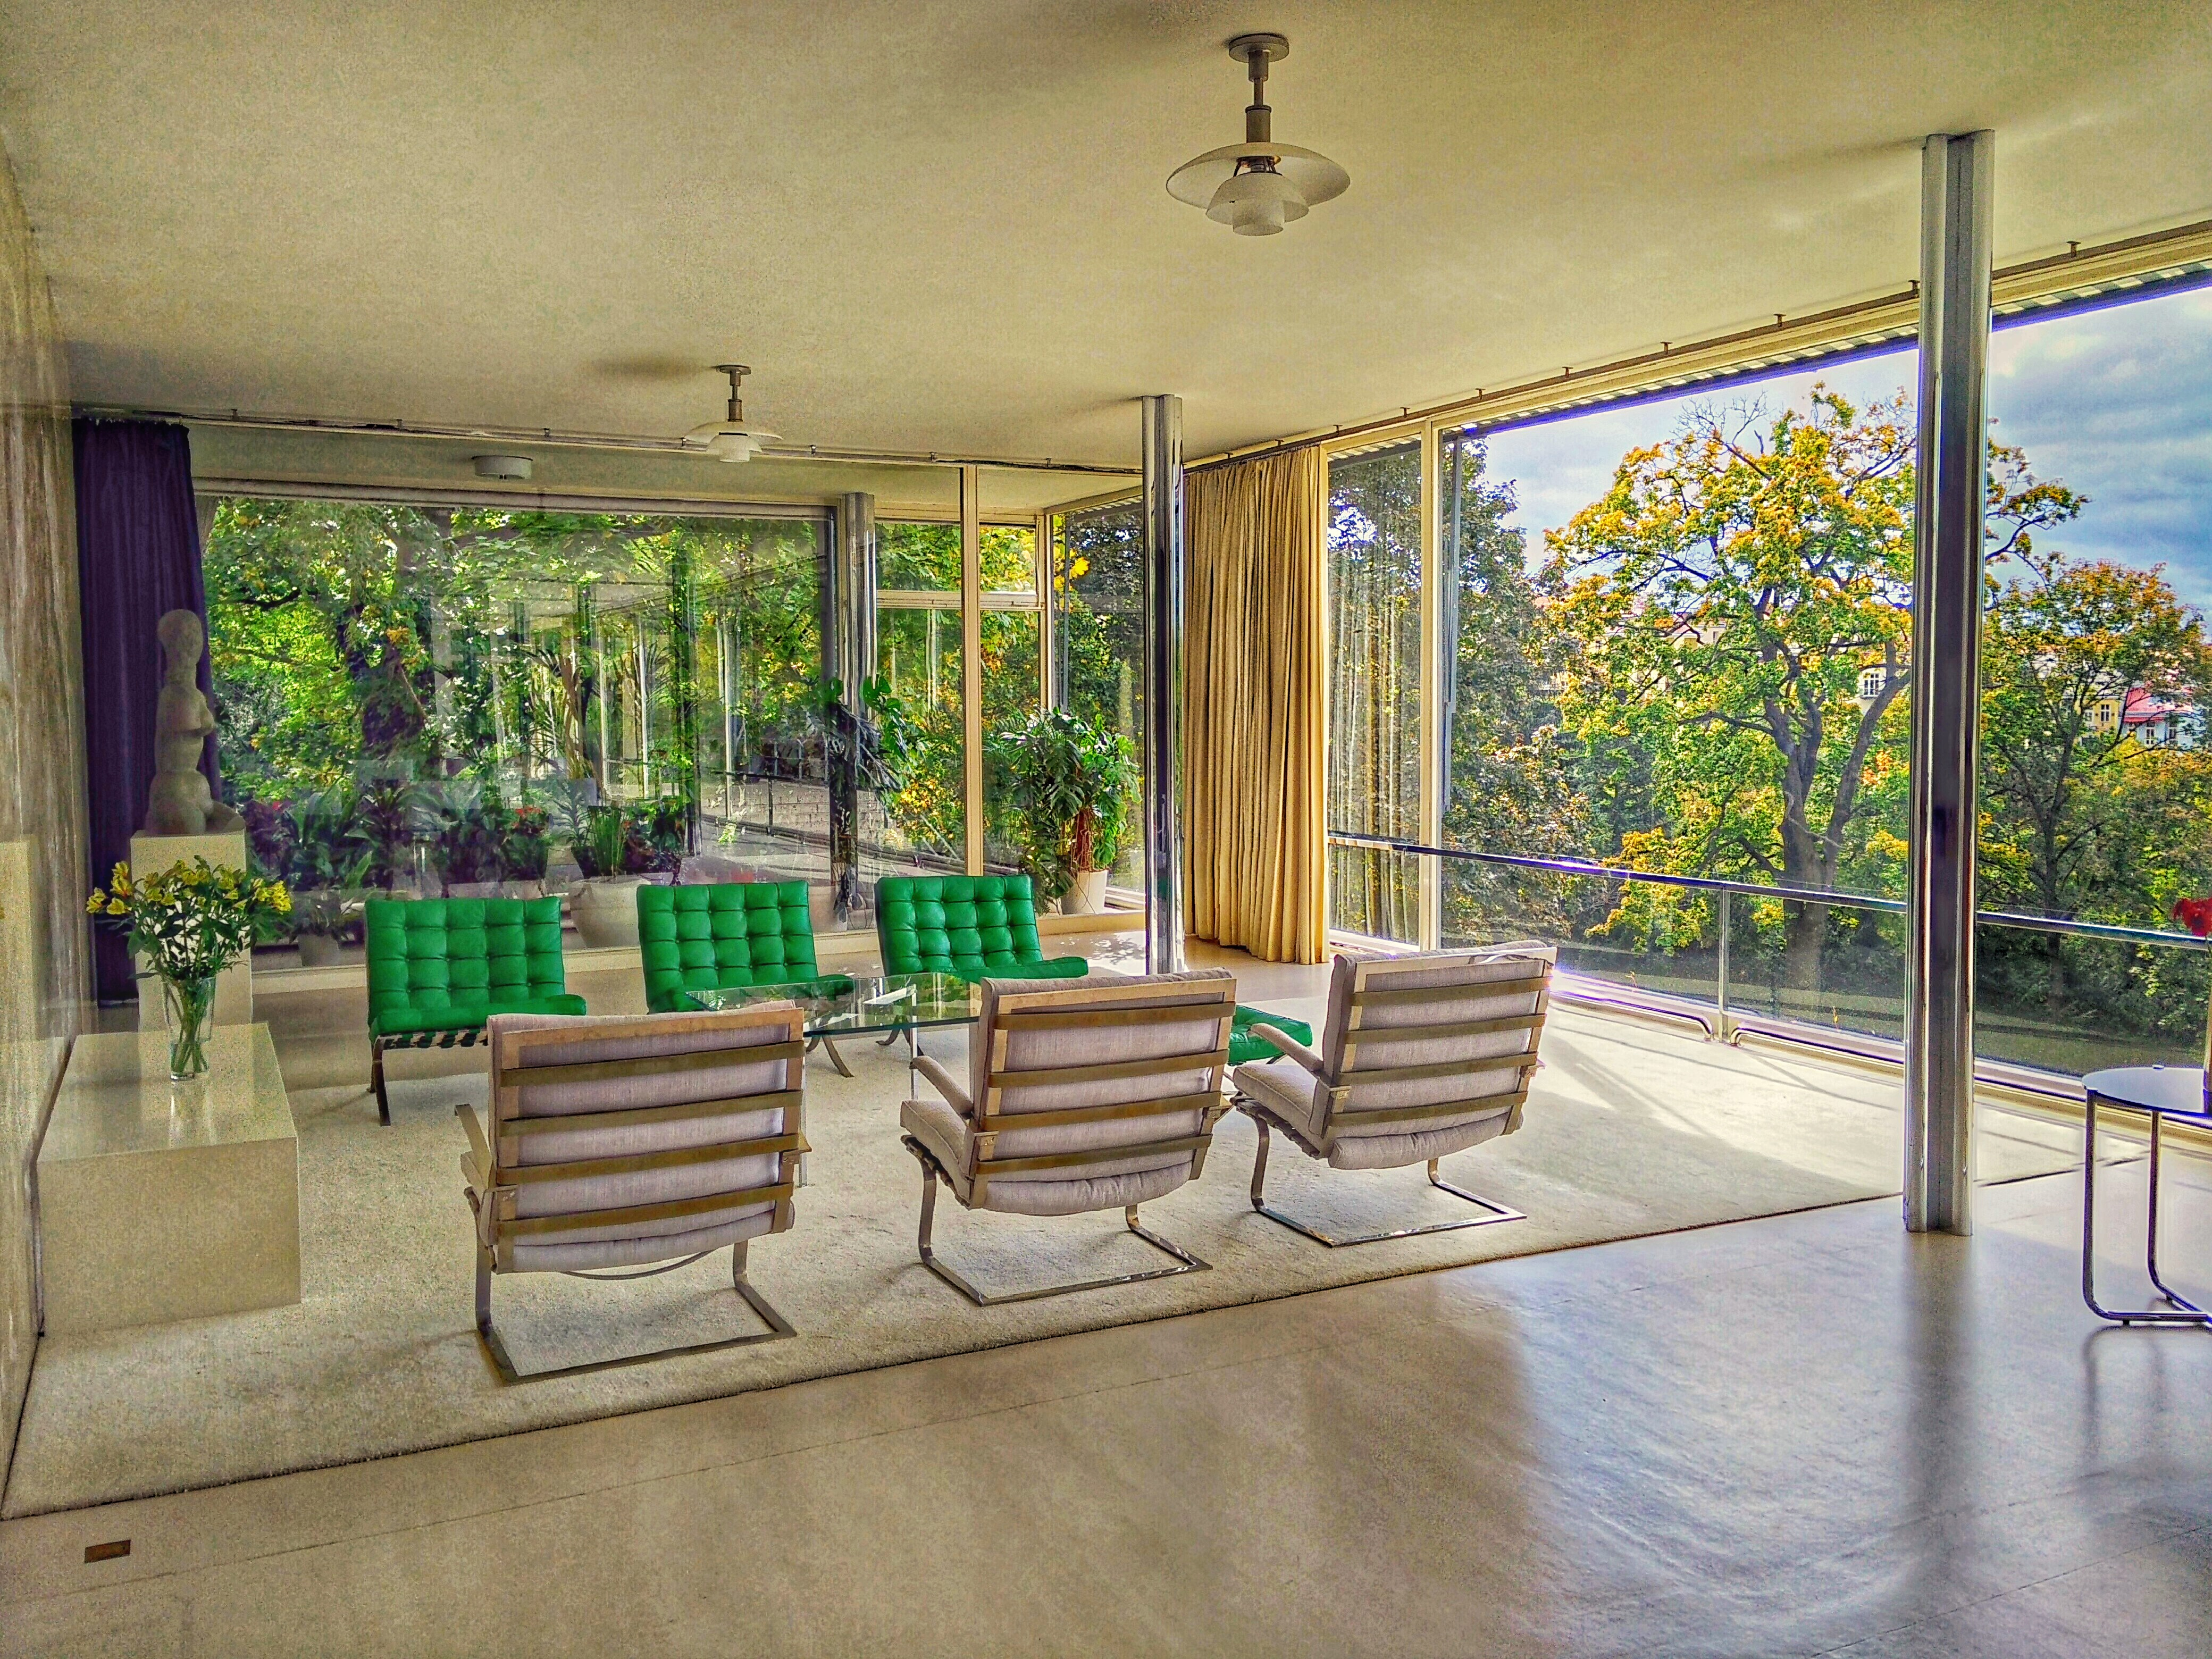
\includegraphics[height=10.7em]{fig/fit-tugendhat.jpg}\\[1em]
\includegraphics[height=10.6em]{fig/fit-sala-house.jpg}\quad
\includegraphics[height=10.6em]{fig/fit-strip.jpg}\quad
% dobravoda - https://cs.wikipedia.org/wiki/Soubor:Kostel_na_Dobr%C3%A9_Vod%C4%9B-Novohradsko.jpg
% strip - denise scott brown: https://www.readingdesign.org/denise-scott-brown-photos/9
% sala - https://en.wikipedia.org/wiki/File:Sala_House_Parents_Realm_1.jpg
% tugendhat - https://www.flickr.com/photos/giverny_com/36877628023/in/photolist-YbKu1P-4J3HtF-4J7XKh-4J3Hxr-2q9AVLT-2k8kJjf-3o6UC1-2mEffFe-ir6bD2-QpB1Mn-jeGrdX-irNkiN-irNP4z-irMjuz-irNjhQ-NevRiJ-2k8goCA-irMMKM-irMQwP-2k8kbWe-2k8kc6Y-2k8kc4J-nVVogH-2k8kcgn-2k8kJaT-2k8kJdt-jeHo7p-2k8kJi8-aeVAve-2k8kJbV-2k8gp9q-anTQqR-irMB3o-irNwHG-Yz6G6D-irMiQZ-2k8kcnE-2k8kJ2G-2oQs2xZ-yuu9bF-jeJuFN-2mcTMdE-5g8KH-nJEuNq-2q9HMf8-5g8Kk-yc9oXq-2mifXPW-2njVnzt-2njVkiz/
% eisenman - https://eisenmanarchitects.com/House-VI-1975
% isokon - https://www.flickr.com/photos/maggiejones/17338557816/in/photolist-2paYN7a-ssgWEj-sq9Db1-4A52rR-NCrec-E3NASp-NBXFf-4nvATQ-4nrxzc-8asA8-tJnxgo-8yckjU-2paYcx9-2paWp7N-aidSyZ-2paWpfD-2paXSBn-2paXSpd-2paXSed-2paYc8r-98yBWx-98BLLY-sspZPP-4vAEkM-ssrJBp-s97oGn-rvrfVm
% selske - https://cs.wikipedia.org/wiki/Selsk%C3%A9_baroko#/media/Soubor:Zbudov3.jpg
\caption{Seven examples that illustrate different approaches to achieving fit.
(1) Vernacular farmhouse in South Bohemia built in the 19th century in the rural baroque style (``selské baroko''),
(2) Church of Our Lady of Sorrows in Dobrá Voda with entrance from the side of the nave,
(3) House VI by Peter Eisenman, bult 1972-75,
(4) Bauhaus-inspired Isokon building in London, built 1929-32,
(5) living space of the modernist Villa Tugendhat by Mies van der Rohe, 1928-30,
(6) the entrance room of the Sala House built by Christopher Alexander in 1983-4, and
(7) 1966 photo of the Las Vegas Strip by Denise Scott Brown from ``Learning from Las Vegas''.}
\label{fig:fit}
\end{figure}

\section{Ways of Achieving Fit}
What I hope to achieve in this text is to document the ways through which architecture can convey
critical understanding and see if those ways let us talk about important issues concerning software. I moved
away from Christopher Alexander, for whom the main question that matters is whether building (or software)
produces living structures in the world.

I think that buildings and software should also raise critical points and much of the above was
exploring some of the ways in which this can be done in software. I would now like to return
to the basic question of how structures achieve good fit. This is a question that Christopher
Alexander studies in detail in his ``Notes on the Synthesis of Form,''\endnote{cite} a book based
on his PhD research written before his work on design patterns. This is, incidentally,
also the text that infuriated Peter Eisenman who than opposed it in his own thesis on formal
analysis of architecture.

According to Alexander, ``every design problem begins with an effort to achieve fitness
between two entities: the form in question and its context. The form is the solution to
the problem; the context defines the problem.''\endnote{notes, p15} According to Alexander,
the problem is that, in anything but the most simple scenarios, ``we cannot give an adequate
description of the context we are dealing with.''\endnote{dtto, p20} The real-world is too
complex and so an attempt to logically deduce the form from a description of the context is bound
to fail. The different methods of achieving fit illustrated in Figure~\ref{fig:fit}
approach this problem differently.

The first approach to the problem is used by vernacular architecture, that is building done
locally, in traditional ways and without guidance of professional architects. We do not need
to appropriate ``charms of fairy-tale countries''\endnote{edited, rudofsky p3 - criticises our condescending
narrative based on talking about exotic countries.} to explain this approach. Aside from
the Musgum mud huts, Alexander talks about New England barns and my illustration is a typical
farmhouse in the southern region of Czechia. The way good fit is achieved in vernacular
architecture is by gradual adaptation. When building a new farmhouse, the local builder follows
the same style as everyone else in the region. Since the needs of most farmers are similar,
this will result in an adequate solution. When the context changes, the building style evolves
gradually by small adaptations. A change is tried in one farmhouse and if it is beneficial, it is
then replicated by other builders. In this mode of working, little is demanded from the individual
builder. ``He need not himself be able to invent forms at all. (...) All that is required is that
he should recognize misfits and respond to them by making minor changes.''\endnote{Notes, p58}
Even if the changes are not improvements, it does not matter. They will simply not be adopted
by others in subsequent buildings.

According to Alexander, the professionalization of architecture destroyed this old process.
However, Alexander also admits that the degree of complexity faced by modern architects is
greater than that of vernacular builders. You cannot build a skyscraper using the method that
works for a farmhouse. Professional architects thus approach the problem by analyzing the context
and inventing a form to fit. This is the modernist methodology, rooted in the maxim ``forms follows
function.''\endnote{Sulivan} Two examples of modernist architecture that illustrate different
variations on the theme above are Villa Tugendhat and Isokon Flats. Villa Tugendhat was built as
a private residence, to create ``a complete vision of luxurious Modernist living.''\endnote{Julia
Jamrozik and Coryn Kempster, Growing up Modern. Childhoods in Iconic Homes, Basel, Birkhäuser, 2021, 83;
quoted in Ana Tost\"oes - Modern Heritage Reuse. Renovation. Restoration (2022, Birkhäuser)}
As such, it featured open plan living space, retractable glazed walls and a floor plan that
reflects the needs of the family, including an easy access through the garage and a separate
driver's appartment. In contrast to the generous space of the Villa Tugendhat, Isokon Flats were
designed as ``minimal flats,''\endnote{Isokon, p60, also note this was theme of the 1929 CIAM congress}
inspired by the question of ``how much space individuals needed to live in comfortably.''\endnote{dtto, p59}
The flats were built for young professional men and women and provided a range of domestic services
and meals made in a central kitchen. The two buildings are daring examples of radical new design
that reflects the changing context. Both of the buildings invent a new form that and aims to
achieve fit by analyzing the context and by emplying technical innovations.

Christopher Alexander developed a range of different approaches to the problem of achieving
fit throughout his career. In ``Notes on the Synthesis of Form'', he suggests that
``we should see the process of achieving good fit (...) as a negative process of neutralizing
the incongruities, or irritants, or forces, which cause misfit''\endnote{Notes, p24} and
he describes an analytical incremental approach that identifies sub-problems (clusters of
interlinked concerns) and gradually resolves those. His later work describes the problem as the
search for what he calls ``quality without a name'', which happens when an environment is
free of contradictions. In the writing on design patterns, Alexander and his collaborators
replace the unwritten knowledge of vernacular architecture with an explicit pattern language.
A good pattern language can then be used to design living structures:\endnote{p134}

\begin{quote}
Each living pattern resolves some system of forces, or allows them to resolve themselves.
Each pattern creates an organization which maintains that portion of the world in balance.
(...) And finally the quality without a name appears (...) when an entire system of patterns,
interdependent at many levels, is all stable and alive.
\end{quote}

The Sala house designed by Alexander shown in Figure~\ref{fig:fit} employs numerous patterns to achieve
the quality without a name. Sleeping is organized in alcoves (involving patterns such as Bed Cluster,
Alcove, Marriage Bed), the house relies on natural light (Tapestry of Light and Dark, Sunny Place),
and the inside of the house is in relationship with the outside garden (Connection to the Earth).
The process relies on an extensive pattern language, which Alexander painstakingly developed with
his co-authors over multiple years. The pattern language is supposed to capture the shared
understanding of the community, which makes it possible to construct agreeable environment.
Alexander's pattern language, however, leads to a particular style of buildings and Alexander
himself later asked whether patterns are enough to generate the living structures he desires.
Moreover, the buildings built using his pattern language are pleasant in a specific way and it is
not clear whether the same approach can be used to construct other types of pleasant
buildings.\endnote{See \url{https://tomasp.net/blog/2022/timeless-way/}}

Christopher Alexander is not the only one who believes that the modernist rational approach
to achieving fit is bound to fail. Robert Venturi, sometimes referred to as one of the founding
fathers of post-modernism,\endnote{he does not agree % https://en.wikipedia.org/wiki/Complexity_and_Contradiction_in_Architecture
and also worked closely with Denise Scott Brown} wrote in his 1966 book ``Complexity and
Contradiction in Architecutre'' that Mies van der Rohe ``makes wonderful buildings only because
he ignores many aspects of a building. If he solved more problems, his buildings would be far
less potent.''\endnote{Complexity and Contradiction, p16} Venturi also cites Alexander
to highlight that problems faced by architects ``increase in quantity, complexity and they also
change faster than before.''\endnote{Complexity and contradiction, p16; citing Alexander's Notes}
But rather than trying to resolve the resulting contradictions, Venturi welcomes them:\endnote{Complexity, p16}

\begin{quote}
I like complexity and contradiction in architecture. I do not like the incoherence or
arbitrariness of incompetent architecture nor the precious intricacies of picturesqueness
of expressionism. Instead, I speak of a complex and contradictory architecture based on the
richness and ambiguity of modern experience, including that experience which is inherent in art.
\end{quote}

In his ``Complexity and Contradiction in Architecture,'' Venturi documents a large number of
examples of architecture that accommodates complexity and contradiction using both historical
examples and his own projects. The church in Dobrá Voda, shown above, illustrates Venturi's point
that the complexity of a site supports richness lacking in purer compositions.\endnote{p28}
The church is built in a village on a hill with a steep slope. Reflecting the site,
the Baroque entrance is from the side of the nave and is visible from the open countryside
that it faces---becoming an appealing landmark.

I talk about Venturi in a section focused on achieving fit mainly because of his later work,
``Learning from Las Vegas''\endnote{cite} written with Denise Scott Brown and Steven Izenour.
The book is a study of the commercial strip, ``important to architects and urbanists today
as were the studies of medieval Europe and ancient Rome and Greece to earlier generations.''\endnote{p.xi (preface)}
For Venturi and his collaborators, the analysis ``is a socially desirable activity to the
extent that it teaches us architects to be more understanding and less authoritarian.''\endnote{p6}

Venturi, Scott Brown and Izenour point out that architects have typically been trying to change
the existing environment rather than enhancing what is already there. The way of achieving
fit with the new complex environment is thus to first understand the existing environment
and its language---and then build with accordance to the language. In the case of the commercial
strip, documented in the book, the language is primarily a language of signs, billboards, arrows
and visual symbols. The ``obvious visual order of the street'' is in contrast with the ``difficult
visual order of buildings and signs.''\endnote{p20} This multi-layered formal structure is not
unlike that of the Hotel Foquet discussed in the previous section.

The authors use the lessons learned as a justification for their own approach to architecture,
which they call the decorated shed. According to this perspective, the architectural form of
the building does not matter that much. A decorated shed is designed and built as a conventional
shelter, reflecting ``proprietor's budget.''\endnote{p13} An additional content is added to
the building in the form of signs---either as literal signs in the case of Las Vegas strip or
as explicit decorations in case of more ordinary buildings. The fact that the authors look
specifically at the commercial strip (and the Levittown suburb in their follow-up work) for
inspiration reflects their acknowledgement of existing American culture---a position that
is shared with the pop art movement. Venturi, Scott Brown and Izenour can thus be seen as
assuming ``the role of servant to society'' whose task ``is to understand and interpret
the wishes of the client.''\endnote{Oppositions, p178} This is in contrast to the modernist
tendency ``to elevant client's value system and/or budget by reference to Art and
Metaphysics.''\endnote{Learning, p102}

The view of Venturi, Scott Brown and Izenour that architecture is ``embedded in a global ideology
from which there is no escape'' is also a negation of the perspective of Peter Eisenman and a
group referred to as ``the New York Five'' who see ``architecture as an autonomous
discourse.''\endnote{Oppositions, 186} This school of architecture offers yet another perspective on
the problem of achieving fit. As I discussed earlier, Eisenman is interested in developing
architectural forms as formal structures, rooted in a formal architectural language and
without direct reference to humanist ideals. His architecture is ``true to its own
logic.''\endnote{\url{https://eisenmanarchitects.com/Fin-D-Ou-T-Hou-S-1983}}
The problem of achieving fit is no longer a driving factor behind architecture, but
something that can emerge as its effect.\endnote{dtto} How less likely this is when compared
to other approaches likely depends on the degree to which the complexity of the problem of
achieving fit, which other architects explicitly try to address, is tractable.

The idea that structures emerging from formal manipulation will find their use is not
exclusive to the proponents of autonomous architecture like Eisenman.
The architectural style known as contextualism also disregards functionalist rationales
and instead recognizes and replicates elements from the local environment. For ``if
Americans won't promenade in urban plazas perhaps they will ice skate in them.''\endnote{Oppositions, p67}

\section{Vernacular Software}

% TODO: Also go through Brand's How Buildings learn for ideas about vernacular buildings

The essential characteristics of vernacular architecture is that it is produced in traditional
ways, without professional architects and that it achieves fit through gradual adaptation.
It typically only needs to address problems of limited complexity. Vernacular architecture
also develops over long periods of time, so its relevance to the world of software is not
immediately apparent. Yet, there are some connections worth exploring.

The web of the 1990s had many of the characteristics of the vernacular architecture and this
fact has been documented in articles and talks by the internet artist and theorist
Olia Lialina.\endnote{Some links to relevant work \url{https://en.wikipedia.org/wiki/Olia_Lialina}}
In her article ``A Vernacular Web'', Lialina describes the web of the mid-1990s as ``bright, rich, personal,
slow and under construction'', but also documents its vernacular nature and its demise:\endnote{Digital Folklore, p19}

\begin{quote}
One could say it was the web of the indigenous... or the barbarians. In any case, it was a web
of amateurs soon to bewashed away by dot.com ambitions, professional authoring tools and
guidelines designed by usability experts.
\end{quote}

\begin{figure}
\centering
\includegraphics[width=0.485\textwidth]{fig/geocities1.png}
\includegraphics[width=0.485\textwidth]{fig/geocities2.png}
\caption{Two examples of typical web pages hosted on GeoCities (viewed using a modern
web browser in an archive maintained by restorativland).}
\label{fig:geocities}
% https://geocities.restorativland.org/SiliconValley/5669/
% https://geocities.restorativland.org/ResearchTriangle/1977/
\end{figure}

% cf. digital folklore reader - https://monoskop.org/images/9/91/Lialina_Olia_Espenschied_Dragan_eds_Digital_Folklore_2009.pdf

The web pages of the mid-1990s were often hosted on the free web hosting service GeoCities, which
offered a simple template-driven web generator or an advanced editor for users familiar with HTML.
Pages were organized in neighborhoods that grouped content by topic, but also simplified discovery
of other content.\endnote{see ``Welcome to the web: The online community of GeoCities during the
early years of the World Wide Web'' chapter} Although the web pages had widely varying content and
graphics, many of them shared a particular style (Figure~\ref{fig:geocities}). They were also
often created using the typical methods of vernacular architecture---by copying existing structures.
In particular, the modular nature of the web meant that ``every line, figure, button and sound was
on its own and could easily be extracted, if not directly from the browser then from looking at the
source code to find the URLs of the files.''\endnote{Folklore, p24} The reusable components of the
1990s web, such as backgrounds, buttons, music and dividers were available from collections
maintained by other users.

Another area where we can find aspects of vernacular way of working is programming, as practiced
by the members of the hacker community at the MIT in the 1960s. The hacker community emerged around
the first available interactive computers, TX-0 and PDP-1. It embraced ideas of openness and
sharing as well as individual ingenuity and skill.\endnote{And it was also mascuiline - see
for example \url{https://dl.acm.org/doi/pdf/10.1145/3451227}} Hackers did not learn programming
through formal education, but through practice and by working with other members of the community.
The hacker culture differs from vernacular architecture in that the problems solved by hackers
were often very challenging and required great individual ingenuity. The ways and the tools
through which they solved the particular programming problems were shared by the community
and improved by a process of gradual adaptation.\endnote{c.f cultures book} There is also a
similarity between the largely unwritten community knowledge of hackers\endnote{HAKMEM}
and the unwritten community knowledge of vernacular builders. The way of working
personified by the 1960s MIT hackers keeps finding its use in various areas of computer programming
to this day.\endnote{Cultures of Programming} However, as a dominant way of building software,
the methods of early computer hackers were replaced with an orderly software engineering
method.\endnote{See cultures, NATO conference}

Both of the above examples share interesting characteristics with vernacular architecture.
They rely on unwritten knowledge shared by a community and also on some notion of copying
and reuse. Whereas in vernacular architecture, it is necessary to copy a form when constructing
new buildings, vernacular web creators relied on literal copying of code, graphics and other
media elements. The fate of those vernacular computing practices also followed the fate of
vernacular architecture. As observed by Alexander, ``with the invention of a teachable discipline
called `architecture,'  the old process of making form was adulterated and its chances of success
destroyed.''\endnote{Notes, p58} The new ``teachable disciplines'' that led to the end of the
vernacular web and vernacular hacker programming were professional web design or user experience
design and the discipline of software engineering, respectively. Both of those replace the
unwritten knowledge and the practice of copying and learning from the community with the
analysis of the context and (re)invention of new forms to fit the context. It is also the case that,
like modern architecture, both modern user experience design and software engineering face problems
of a greater scale and complexity.

When Bernard Rudofsky organized the exhibition ``Architecture Without Architects'' that popularized
the term ``vernacular architecture'' in 1966, he was one of the first to recognize that our
attitude to traditional architecture ``is plainly condescending'' and that:\endnote{Rudofsky, p3 and p4}

\begin{quote}
There is much to learn from architecture before it became an expert's art. The
untutored builders in space and time (...) demonstrate an admirable talent for
fitting their buildings into the natural surroundings.
\end{quote}

Architects and designers have, since then, learned to recognize the value of vernacular and
indigenous architecture.\endnote{e.g. lo-tek book} I believe that computer scientists and
programmers should similarly look to their vernacular past for interesting ideas.\endnote{See
also complementary science, BASIC; some work in this area e.g. people's history, dot-com design.}

\begin{figure}
  \centering
  \includegraphics[width=0.7\textwidth]{fig/spacewar.jpg}
  \caption{The Spacewar! game, created by the MIT hackers, running on a restored PDP-1 computer
  in the Computer History Museum}
  \label{fig:spacewar}
  % https://www.flickr.com/photos/toasty/364960084/in/photolist-yfvVf-bcqPmP-6VT4Pi-cL97ay-5VP2F3-fAMdVr-515UAU-Dk8Bk6-pNfx2r-7jfCxZ-5EgWhd-bqJVp2-bqJW3K-bqJVPT-bqJVKH-bqJVWr-bqJVf6-bqJW7z-bqJVDR-bqJVte-bqJWhH-38dxUF-bqJVyZ-4vP5DW-bqJWct-i7nQzA-bqJVjX-9e8B4L-AAF4-8HP4BV-4W5x5u-2E5ZNT-dDyBmF-4JVL4h-63tUoA-txw4N-9e5wcZ-4Ro5GJ-4o17j-oxWix-9e5w2a-9oN8SW-b47ZUP-9sXFJF-RFArzN-4n4zRY-jS4Q6K-7jNnMV-NTpPj-2PWG1
\end{figure}

The vernacular web culture is perhaps closer to the pop signs of the commercial vernacular
of Las Vegas than to rural vernacular praised by Alexander. In any case, it developed into a unique
creative culture and the GeoCities service itself hosted over 38 million pages by the time it was
shut down in 2009, most of which were created by enthusiasts and non-professionals. How exactly
this was achieved would be a subject of a fascinating socio-technical study of the era, but
there are some easily identifiable technical factors that enabled this. First, the GeoCities
template-based web page generator made it easy for users to get started, but it did not restrict
them. There was a natural transition from a novice user to someone who can fiddle with the
HTML source code, modify it and, through this process, gradually learn more about the technology.
Second, the modularity of the early web made it easy to copy and reuse aspects of other sites.
This included graphics and media, but also parts of the HTML markup and, later, JavaScript code
that was often used to implement ``pop'' visual effects such as rollover (changing an image when
a mouse cursor is over it) or mouse followers (element that follows the mouse cursor).

The technical characteristics that enabled the vernacular web could well be built into new
programming systems. The first requirement is that there should be gradual progression from
an end-user to a novice and, eventually, to an expert. This requires transparency. When a
simple user-friendly tool guides you through the creation of new content, you still need to be
able to see (and interactively engage with) the underlying representation, or source code, of
the result. The same transparency is necessary for sharing of knowledge in the community.
When a user finds some component or behavior interesting, they need to be able to locate its
implementation, copy it (easily extracting only the relevant parts) and reuse it. The domain
where this is perhaps most needed is educational software. And systems such as Scratch let
you explore the gallery of other users' creations, see inside them and ``remix'' them
(although extracting and copying components is still challenging).

The programmers of the 1960s MIT hacker culture illustrate another characteristic of
vernacular architecture mentioned above---an adminarable talent for fitting their software
into their technical environment. An example that illustrates this is the Spacewar! game
(Figure~\ref{fig:spacewar}) that was built to showcase the technical capabilities of the
PDP-1 computer. The initial version of the game featured two spaceships with thrust, shooting
torpedos at each other. Additional ideas proved challenging to implement. Adding gravity and
realistic star map required inventing clever programming tricks such as compiling a special-purpose
program at the start of the game to rotate the spaceship.\endnote{on rotation see
\url{https://nideffer.net/classes/135-09-F/readings/rolling_stone.html}, for more also spacewar
chapter in you are not expected to understand this.}

\begin{figure}
  \centering
  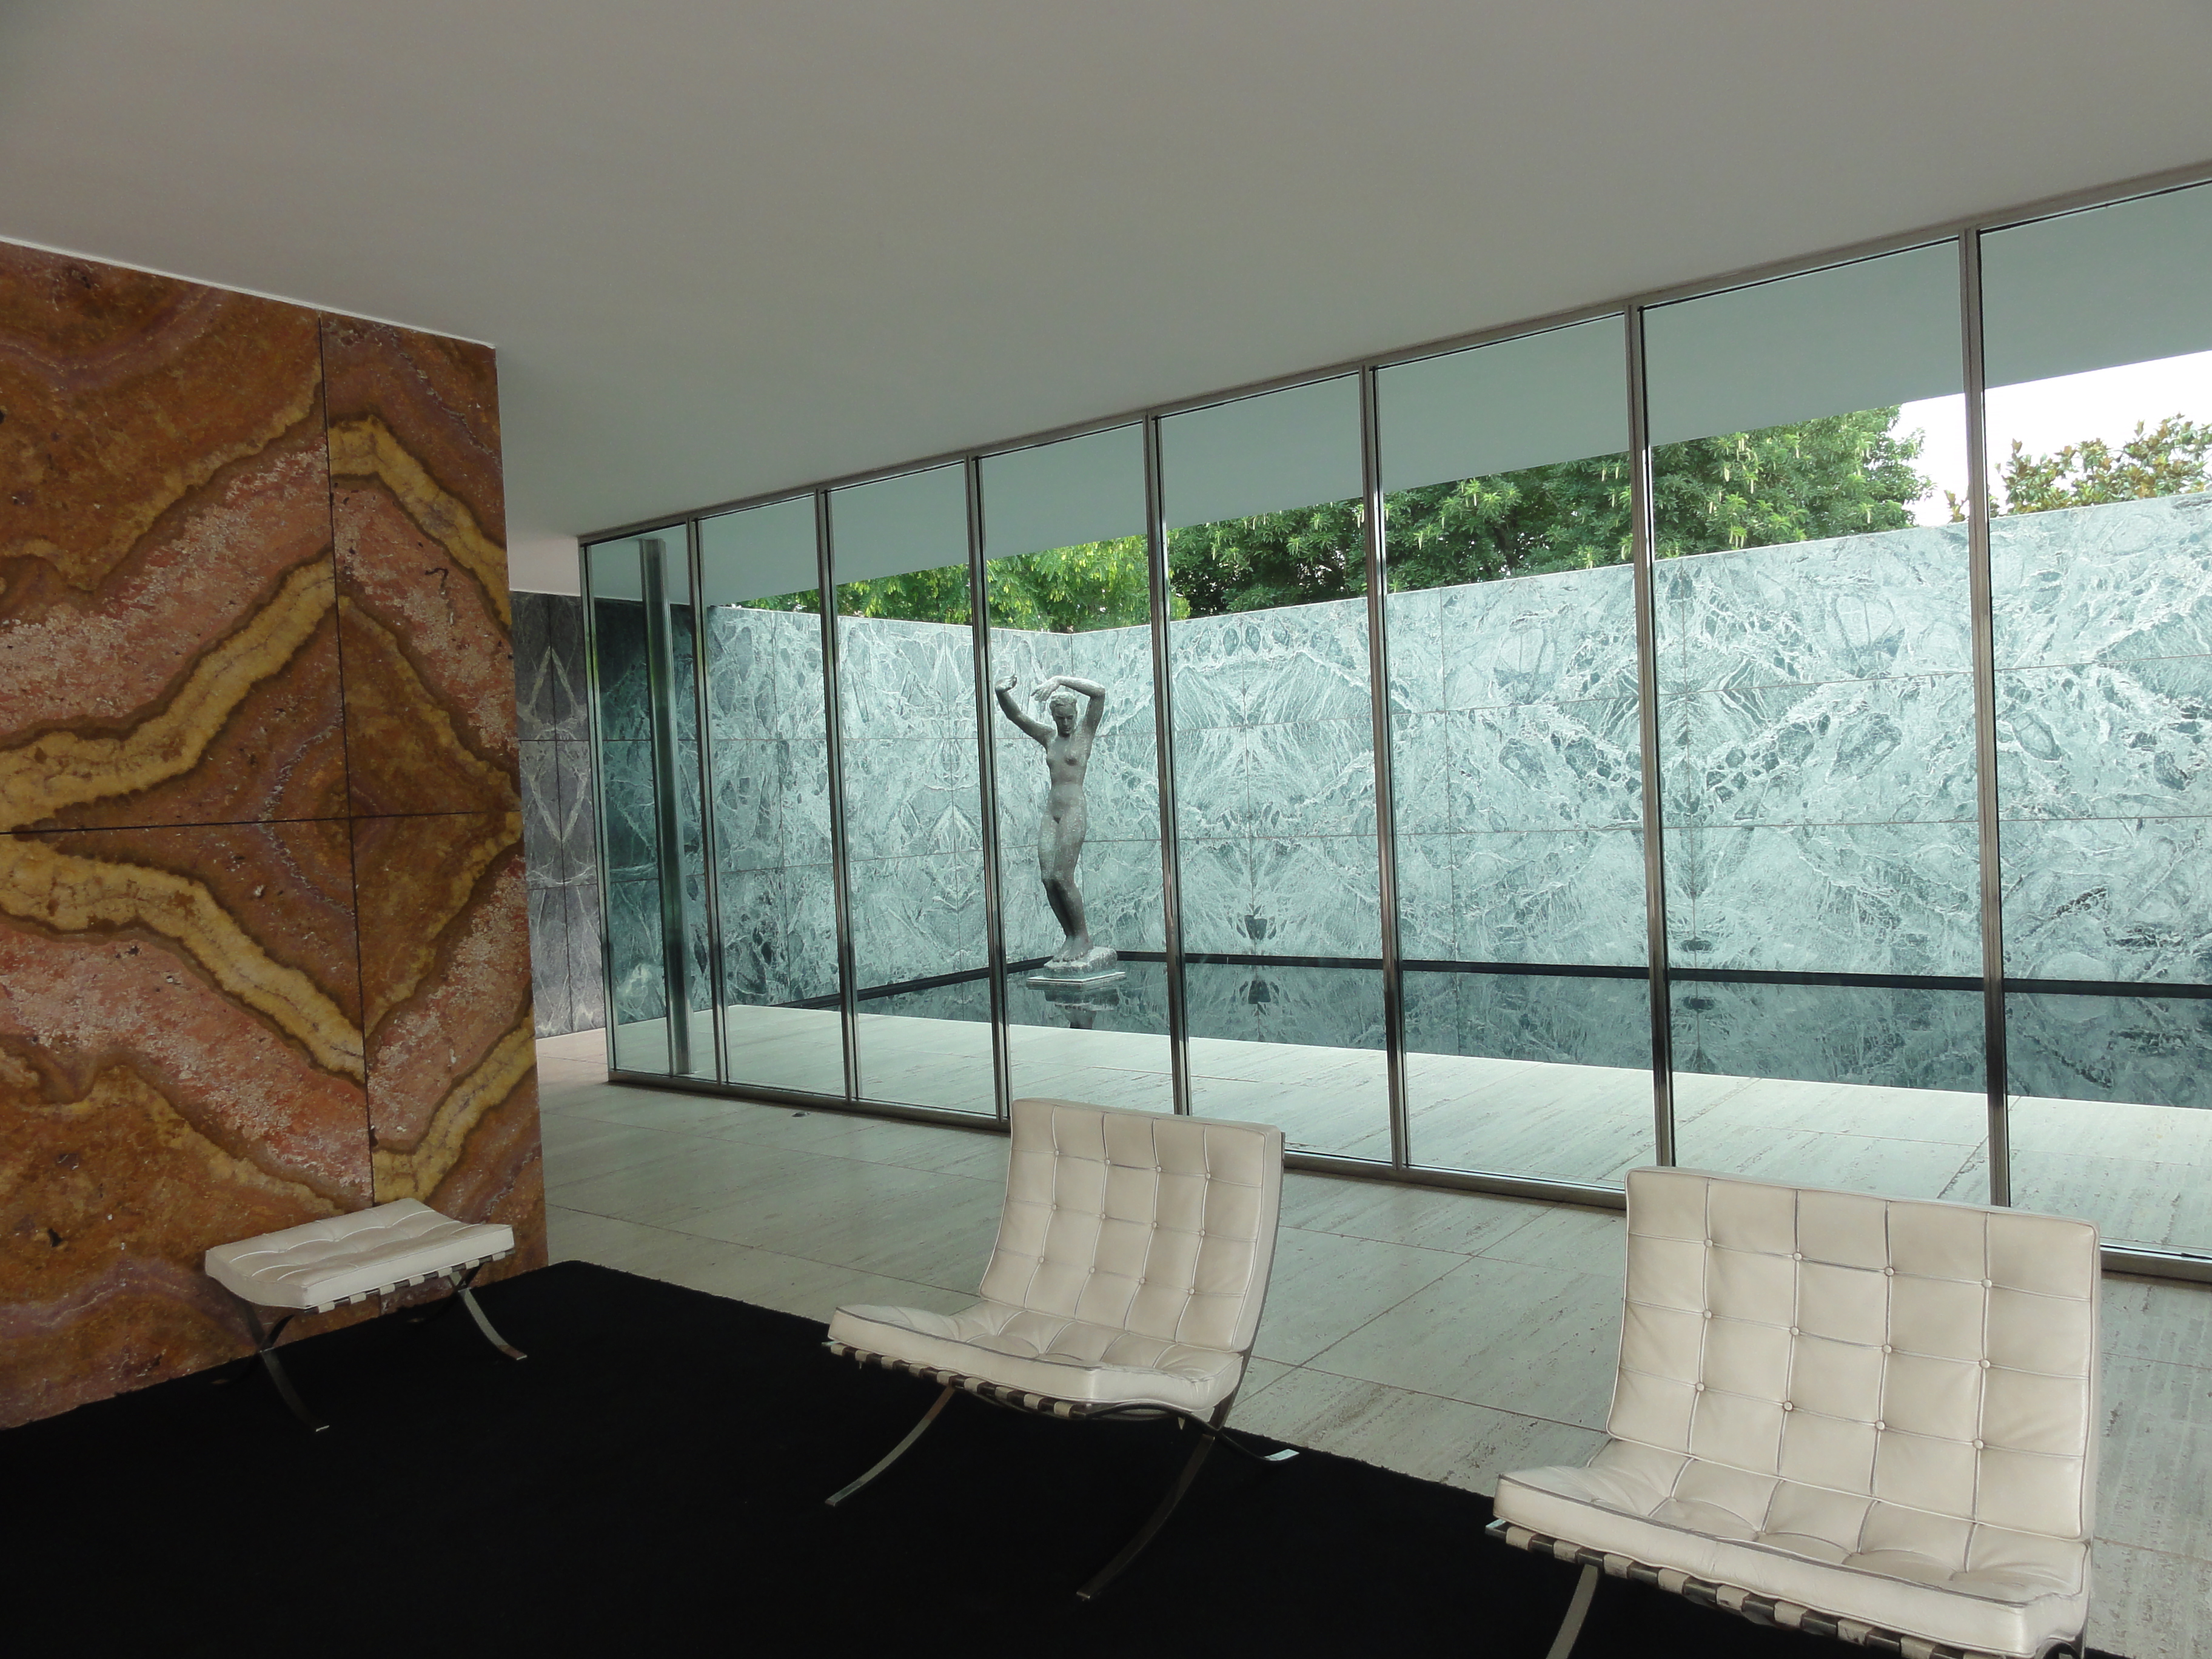
\includegraphics[width=0.6\textwidth]{fig/barcelona.jpg}
  \caption{Replica of the Mies van der Rohe pavilion, rebuilt in 1986 after the 1929 orginal.}
  \label{fig:spacewar}
  % https://www.flickr.com/photos/toasty/364960084/in/photolist-yfvVf-bcqPmP-6VT4Pi-cL97ay-5VP2F3-fAMdVr-515UAU-Dk8Bk6-pNfx2r-7jfCxZ-5EgWhd-bqJVp2-bqJW3K-bqJVPT-bqJVKH-bqJVWr-bqJVf6-bqJW7z-bqJVDR-bqJVte-bqJWhH-38dxUF-bqJVyZ-4vP5DW-bqJWct-i7nQzA-bqJVjX-9e8B4L-AAF4-8HP4BV-4W5x5u-2E5ZNT-dDyBmF-4JVL4h-63tUoA-txw4N-9e5wcZ-4Ro5GJ-4o17j-oxWix-9e5w2a-9oN8SW-b47ZUP-9sXFJF-RFArzN-4n4zRY-jS4Q6K-7jNnMV-NTpPj-2PWG1
\end{figure}

Aside from illustrating a unique degree of fit achieved by the vernacular programming practices
of the hackers, the Spacewar! example lets me illustrate another interesting parallel with
architecture. In architecture, some of the most radical ideas appear in structures that are not
regular buildings. This includes monumnets and follies, exhibition pavilions or stage sets.
The ironic column in the 1980 Venice Bienale was one example I mentioned earlier. Another is
the German pavilion built by Mies van der Rohe for the 1929 International Exposition in Barcelona,
which exhibited the open floor plan and column-supported roof that we saw just six years later
in the Villa Tugendhat.\endnote{An Accidental Masterpiece: Mies van der Rohe's Barcelona Pavilion}
In the world of software, demonstrations are one kind of software that plays a similar role.
The special context of software demonstrations makes it possible to use them for playful purposes
or to illustrate specific technical abilities---such as running an interactive game with gravity
and realistic star map on a 730kg computer with a total memory of 4,000 of 18-bit words.

% TODO: Maybe think about vernacular programming languages? like PHP

It may be interesting to use the lens of vernacular architecture to look at the development
of programming languages too. As documented by Leo Meyerovich and Ariel Rabkin,
``the original designers of today’s popular languages are typically not experienced in programming
language design.''\endnote{Socio-PLT: principles for programming language adoption}
This alone does not make them vernacular, but the languages are often created in the
software equivalent of ``the most complicated configurations in the landscape.''\endnote{Rudofsky, p4}
In words of Meyerovich and Rabkin, ``a common pattern is for programmers with expertise in other
domains to create a language when they perceive an unmet need.''\endnote{socio-plt}
Programming languages not designed by programming language designers often achieve their
fit by solving a more specific problem that is initially perceived as simple. They can even be
well-optimized for the initial specific problem. What they lack, or exhibit only in a limited
form, is the gradual adaptation. In case of programming languages, this is typically prevented
by the fact that once a language gains some users, it becomes impossible to change it.

Perhaps if each software project had to start by creating its own programming language---just
like each farmer needs to build a barn---we would eventually get a vernacular programming
language, highly optimized for its environment!

\section{Modernism of Conceptual Coherence}

It would be simplistic to reduce modernist architecture to the problem of achieving fit.
As we saw above, modernist architects were interested in finding and supporting new modern ways
of living. But this often came together with the need to find new architectural forms.

The way of thinking about software that comes the closest to modernist architecture is
the notion of conceptual integrity, developed by Fred Brooks in his influential book
``The Mythical Man-Month''.\endnote{cite} As with modernist architecture, conceptual integrity
is not merely about achieving good fit or developing a system according to its specification.
It is also about internal logic and clarity of the involved structures:

\begin{quote}
Every part must reflect the same philosophies and the same balancing of de\-siderata.
Every part must even use the same techniques in syntax and analogous notions in semantics.
Ease of use, then, dictates unity of design, conceptual integrity.\endnote{Brooks, p44}
\end{quote}

Even though Brooks talks about internal consistency of the design, the motivating factor
is function. It is not---as with architects exploring formal grammars---internal consistency
of formal structures detachd from the reality. But for ``a given level of function, (...) that
system is best in which one can specify things with the most simplicity and
straightforwardness.''\endnote{dtto, p44}
In software, the problem of achieving internal consistency is as tricky as the problem of achieving
fit between the form and the context in architecture. Brooks believed that it is possible to
achieve conceptual integrity if the design proceeds ``from one mind, or from a very small number
of agreeing resonant minds.''\endnote{Brooks, p44}

Interestingly, the modernist methodology in the world of software also partly responded to
the newly emerging ``modern'' ways of using software. The Mythical Man-Month was published
in 1975. It reflected the author's experience of working on the operating system for the
new IBM/360 line of computers. However, it also appeared a couple of years after other two
major developments in the software industry. One was the 1968 NATO conference on Software
Engineering that introduced the very term ``software engineering'' and is sometimes seen as
marking the move from the ``black art of programming'' to the new science of ``software
engineering''.\endnote{documented in cultures; ensmenger etc.}

Another development was related more to the way computers were employed by businesses.
The influential McKinsey report ``Unlocking the Computer's Profit Potential''\endnote{cite}
published in 1968 argued that many ``large companies have successfully mechanized the bulk
of their routine clerical and accounting procedures'' using computers. According to the report,
most companies were only slowly realizing that the ``second stage of the computer revolution,
unlike the first, entails real operational changes.''\endnote{report in magazine
\url{http://www.bitsavers.org/magazines/Computers_And_Automation/196904.pdf}, p30}
In other words, the managers responsible for the use of computers need to move from simple
automation of existing processes to finding new ways of utilizing computers in their companies.
I would argue that there is a similar interplay in this development as in the modernist
architecture. Just like modernist architecture reflected and enabled new modern way of living,
new modernist approach to software development has been interconnected with new modern ways
of using computers from the 1970s onward.

The software development methodologies of the 1970s are now perhaps more obviously outdated
than the modernist architecture of the 1930s. What followed them---and to what extent can the
different alternatives be related to various post-modern tendencies in architecture---would be
an interesting question to explore further. There may be some interesting analogies.
I will look at ideas inspired by formalism of Eisenman and post-modernism of Venturi later.
Concerning development methodologies specifically, many of the later developments learned to
better acknowledge the ``complexity and contradiction'' involved in the typical sofware project.
Distributed open-source development methodologies characterized by Raymond in ``The Cathedral and
the Bazaar''\endnote{cite} emerge from complex social structures, but are at least as effective
as Brooks' ``one mind''; the Agile development methods aim to achieve fit by gradual adaptation
and would be closer to vernacular methods praised by Alexander.

% READ: Form follows fiasco: https://archive.org/details/formfollowsfiasc00blak/
% (and see other reflections on the failure of modernism in Jencks, p29)

Critics of modernist architecture and modernist urban planning pointed out a number
of its limitations. Many of those are also relevant for software. One of them has been
pointed out by French architect and theoreticiaan Bernard Tschumi:

\begin{quote}
While the puritanism of the Modern Movememnt and its followers has often been pointed out,
its refusal to recognize the passing of time has rarely been noticed. (Not surprisingly,
glass and glazed tiles have been among the preferred materials of the movement---for
they do not reveal the traces~of~time).\endnote{oppositions, p360}
\end{quote}

Software systems do not decay in the same literal way as the materials used in buildings
(there is no plaster falling off the concrete blocks of the software equivalent of the
Villa Savoye as discussed in Tschumi's article). The kind of decay that software faces is more
often caused by changes in its environment, that is the context that initially shaped the form.
In the world of software, the requirements change as the situation in the real world that the
software responds to changes, the technical platforms and systems on which software runs change,
programming languages and styles evolve and components the software is built from change
(npm packages being the most notorious example).

Modernist software is not built to adapt well, just like most modernist buildings are not
built to adapt well. Modernist architecture ``made the profound mistake of taking a
snapshot of the high-rate-of-change `organic life' within building and immobilizing it
in a (...) low-rate-of-change structure and skin of the building.''\endnote{Brand, p157}
Or as Stewart Brand puts it ``The credo `form follows function' was a beautiful lie.
Form froze function.''\endnote{dtto} The possibility of designing more adaptable building,
as well as more adaptable software, is an interesting problem that I will return to later.
(In particular, I want to see if there could be a software equivalent of Brand's ``material
that looks bad before it goes bad,'' i.e., a way of building software where the material
warns us about likely imminent structural faults.)

\begin{figure}
  \centering
  \includegraphics[width=0.9\textwidth]{fig/pruitt-igoe.jpg}
  \caption{The demolition of the second Pruitt–Igoe building, April 21, 1972.}
  \label{fig:pruitt}
  % https://en.wikipedia.org/wiki/Pruitt%E2%80%93Igoe
\end{figure}

Whereas the failures of modernist architecture were typically limited to individual buildings,
the failures of modernist urban planning---rooted in the same principles of rational
planning---were more high-profile. An iconic example has been a large housing project,
built as part of urban renewal projects, often to replace former slums. The demolition
of one such housing project, Pruitt-Igoe in St Louis, in 1972 has been labelled as the
day modern architecture died by architectural critic Charles Jencks (Figure~\ref{fig:pruitt}).
We can see the housing projects as monumental scale follow-ups to the modernist Isokon building
that I examined earlier---and the monumental scale, as well as very different socio-economic
conditions, is likely why their fate was different.

The foremost critic to oppose the modernist urban planning was Jane Jacobs. In her 1961 book,
``The Death and Life of Great American Cities,''\endnote{cite} Jacobs looked closely at
the street life in Greenwich Village and Boston's North End neighborhood at the time and
documents what makes them work. This includes lively mixed-use, dense population and
``eyes on the street'', as well as diversity of buildings and diverse population. That is,
properties that were mostly absent in modernist housing projects. Jacobs' analysis
raises a number of questions about software, some of which I explored
elsewhere such as:\endnote{Programming as Architecture, Design, and Urban Planning}
If the rational structure does not produce working software, what are the characteristics
of software and programming systems that actually do it?

One interesting inquiry into the modernist urban planning came James C. Scott who identifies
modernist patterns---similar to those of modernist urban planning---in a range of other
areas of society including forestry, agriculture and politics. However, many of the modernist
structures that Scott talks about find some way of working. In Scott's account, this is often
enabled by ``dark twins'', that is inofficial structures that exist hidden from the official
modernist view that arise ``to perform many of the various needs that the planned institution
fails to fulfill.''\endnote{Scott,p261} One personification of the concept of dark twin,
documented by Scott is the East German factory worker, touring the country in his Trabant
auto to secure key missing parts not available through official channels, in exchange for
valued goods such as fashionable clothes or champagne, purchased using factory funds.\endnote{p350}
(Another example would be the illegal freelance engineer Archibald Tuttle in Terry Gilliam's
movie Brazil.)

% Other dark twins:
% * Comments in listings package docs
% * Stack overflow as replacement for docs

\begin{figure}
\begin{lstlisting}[language=ts]
// Recursively retrieves a nested value from an object using a path
function getValueByPath(obj: any, path: string[]): any {
  if (path.length === 0) return obj;
  if (typeof obj !== "object" || obj === null) return undefined;
  const [key, ...restPath] = path;
  return getValueByPath(obj[key], restPath);
}

// JSON data could come from external source
const sample = '{ "user": {
  "name": "Bup",
  "address": { "city": "Prague", "zip": "17000" }
}}';
const parsed = JSON.parse(sample);

// Access nested object members dynamically
getValueByPath(parsed, ["user", "name"]);
getValueByPath(parsed, ["user", "address", "zip"]);
\end{lstlisting}
\caption{A TypeScript example using the \texttt{any} type to dynamically process JSON input.}
\label{fig:any}
\end{figure}

The idea of dark twins raises a question about software design as well. To parphrase Scott---to
what extent is successful modernist software design parasitic on similar informal processes that
it cannot create or maintain?\endnote{p6}

I believe one illustration of the above is the type system of the TypeScript language.
(More specifically, I will consider earlier versions of the language. In later versions, the
understanding of types in TypeScript has evolved.) The type system of early TypeScript
featured many types that are common in type systems of more pure languages: primitive types,
object and interface types, function types, union types and generic types. Those are useful
for much of ``modernist'' code that operates on clear and well-defined structures. But not
all code is like that. All programs also need to work with some kind of external data
(Figure~\ref{fig:any}) and this cannot easily be done using purely modernist type system.
TypeScript solved the problem by also including a dark twin---the \texttt{any} type. The type
breaks the pure modernist properties of the type system (the system cannot guarantee any safety),
but its inclusion was likely crucial for the adoption of TypeScript. The system could actually
be used in practice to work with data and interoperate with the JavaScript ecosystem.

The evolution of the TypeScript type system deserves a further analysis. Later versions
continued adding features that reflected typical (non-modernist) coding patterns
in JavaScript. As the number of dark twins in the system grew, they became integrated into the
official structures of the type system---so what started as modernist design with the necessary
supporting dark twins may have evolved into a post-modern assemblage.

\begin{figure}
  \centering
  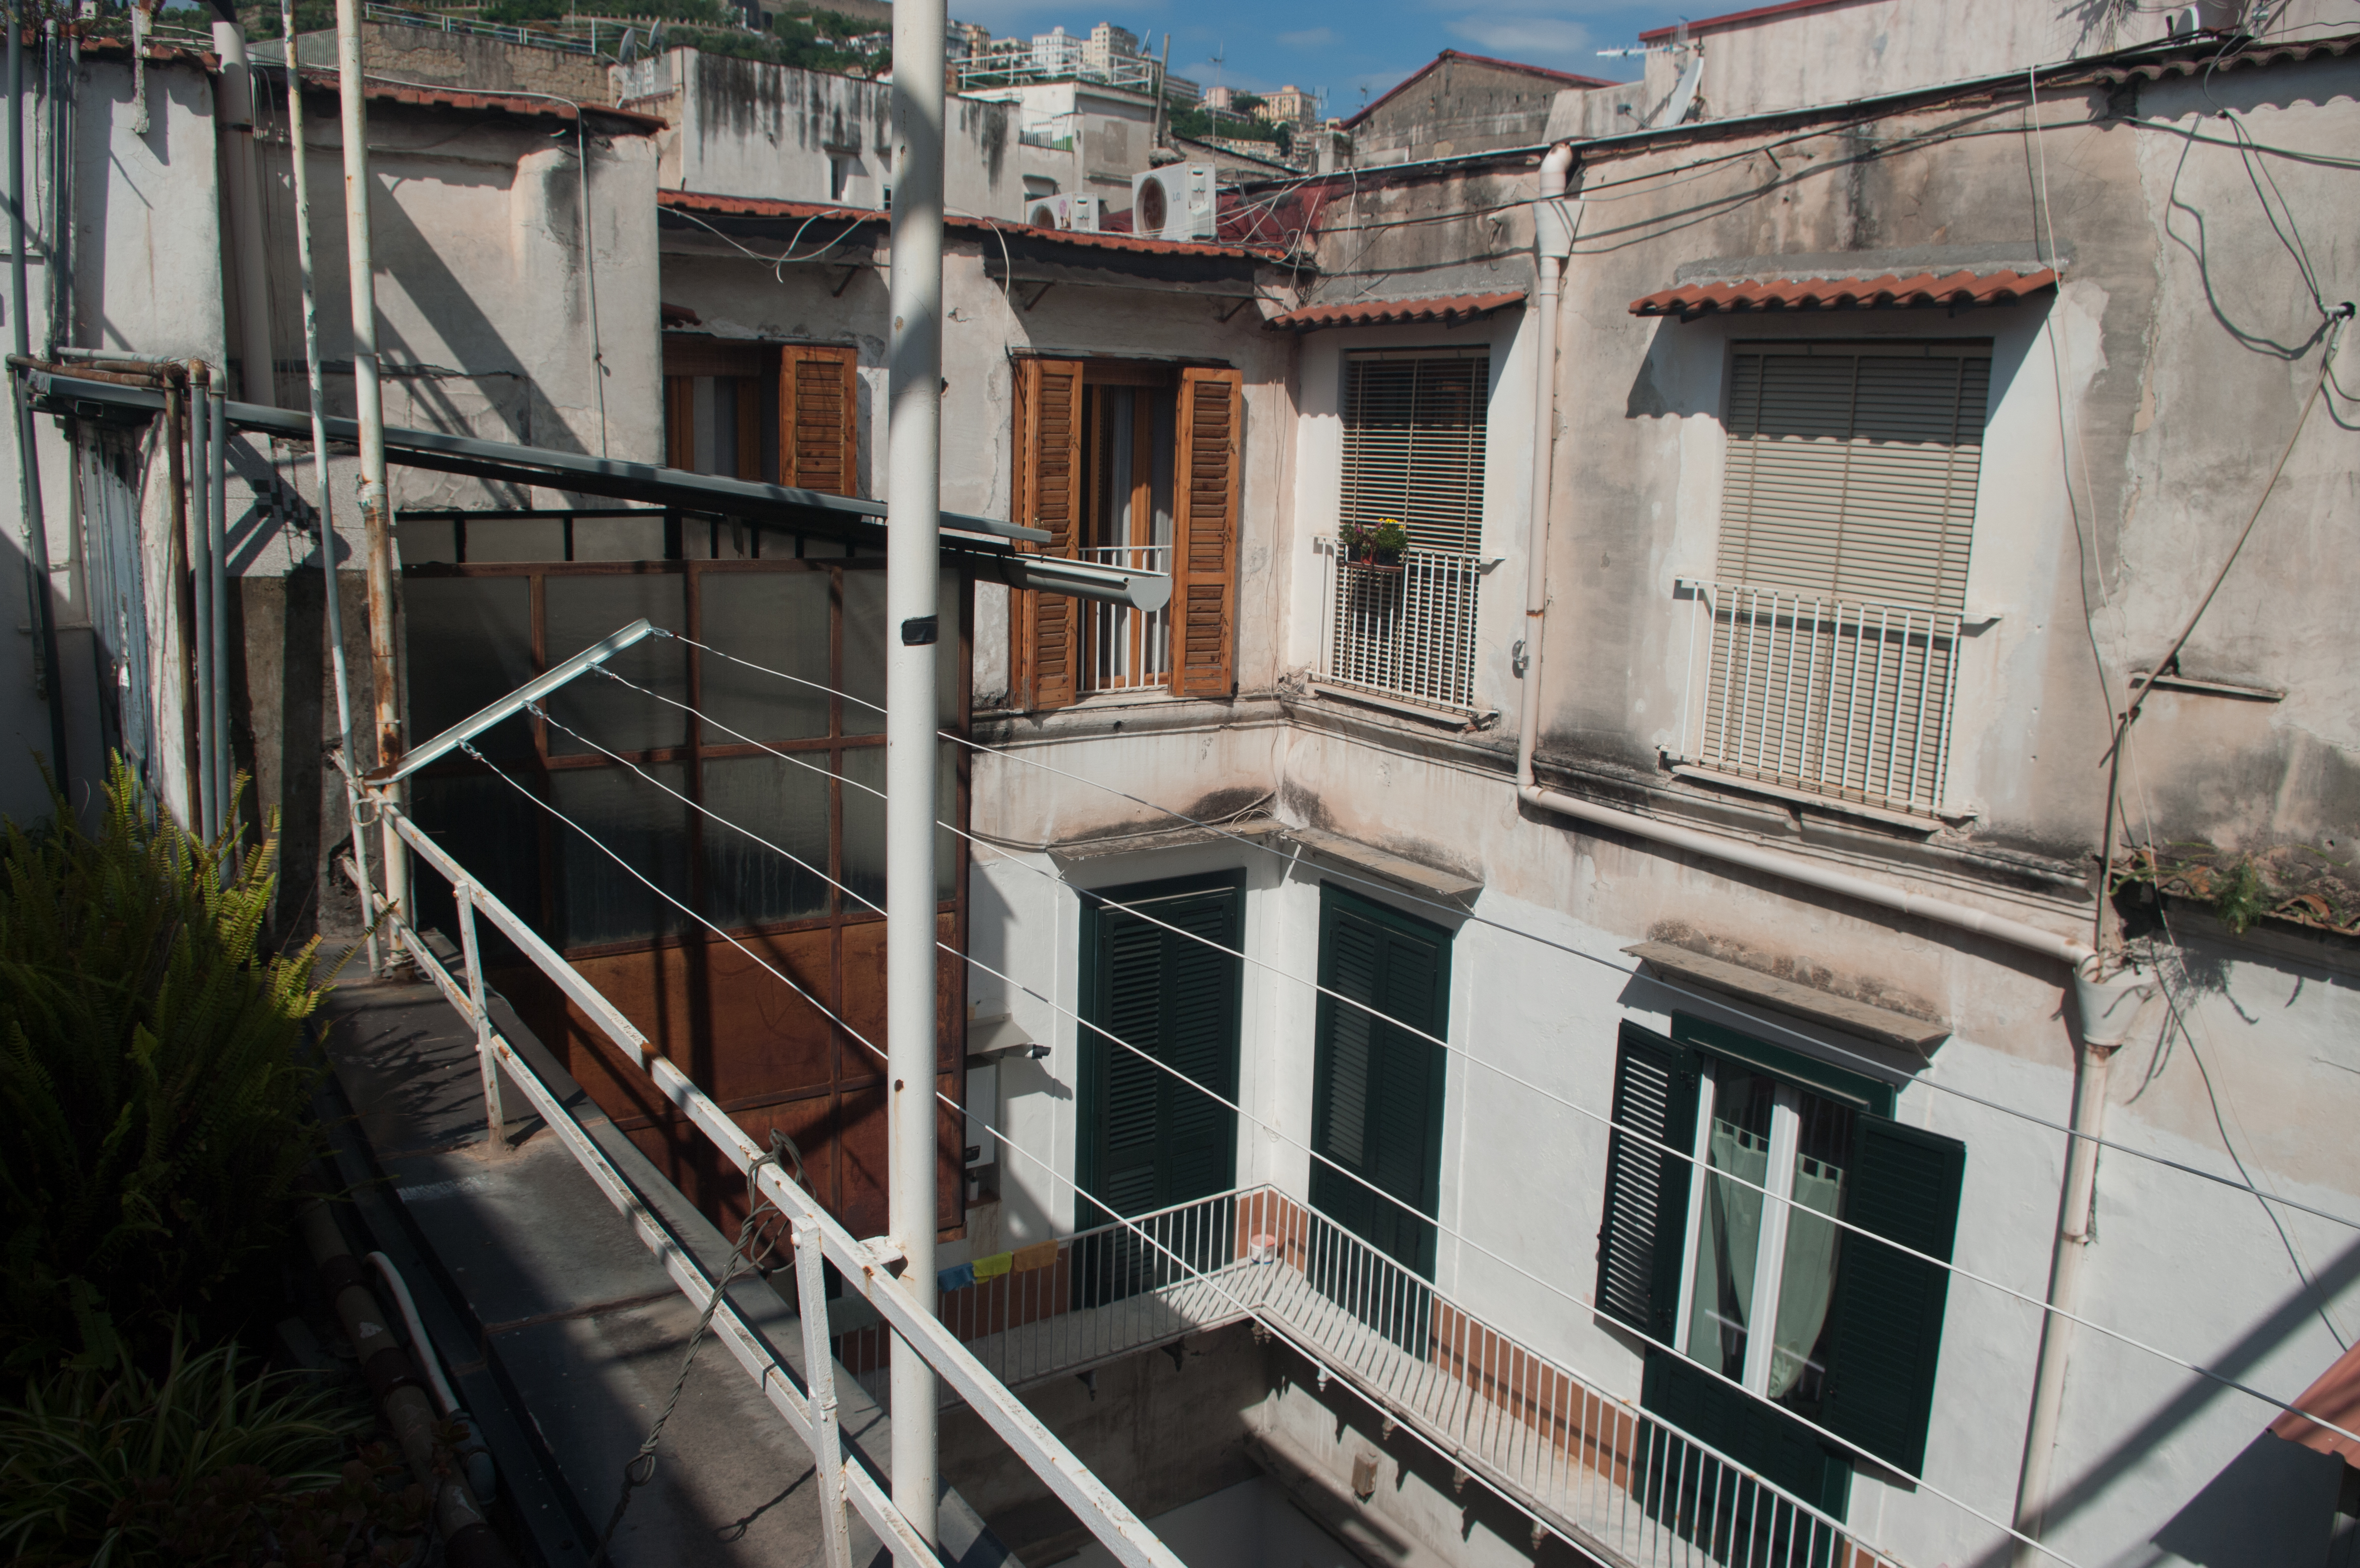
\includegraphics[width=0.85\textwidth]{fig/palazzo.jpg}
  \caption{Additonal floors and other additions on the top of a 19th century palazzo in Naples}
  \label{fig:palazzo}
  % own
\end{figure}

\section{Complexity and Contradiction in Software}

The TypeScript story that I hinted at in the previous section may serve as an illustration of an
important fact. In the earlier versions, we could read the language as being based on modernist
design, featuring strong rational type system. There were some unavoidable dark twins, necessary
to make the design practical, but those were only (somewhat) reluctantly admitted. However, the
later versions of TypeScript seem to acknowledge and embrace the complexities and contradictions
inherent in the system, which combines some aspects of initial rational design with the many
complexities of the environment and perhaps also whims of the most recent JavaScript framework
creators.

Should programmers and computer scientists embrace complexity and contradiction in software,
in ways that are similar to those advocated by Robert Venturi for architecture? First, there
is a certain honesty in acknowledging complexity and contradiction in cases where it cannot
be avoided. Venturi himself also does not argue for introducing unnecessary complexity. He says
that ``abstruse architecture is valid when it reflects the complexities and contradictions of
content and meaning.''\endnote{Complexity, p25} Venturi praises a number of benefits
of working with this fact.

The fact that contradictions support ``richness'' in design (as illustrated by the church in
Dobrá Voda above) is perhaps primarily aesthetical and not necessarily of interest for software
designers. Still, working in an atypical context may serve as a source of inspiration for novel
design. For example, many of the interesting aspects of the Erlang programming langauge arise
from the fact that it was initially designed for telephony applications, which are highly
concurrent, distributed and must be fault tolerant, supporting change ``on the fly'' without
a loss of service during update.\endnote{From ``A History of Erlang''}

Another interesting observation about complexity made by Venturi is that complexity is robust.
It provides an answer to the criticism of modern design that I mentioned in the previous section.
Whereas ``one foreign element casts into doubt the entire effect of some modern
buildings,''\endnote{p42} a ``good deal of clutter'' and renovations does not destroy the
Italian urban scene of many times adapted and reconstructed palazzi (Figure~\ref{fig:palazzo}).
This seems to be the case about programming languages too. Consider the C++ language as an
example. ``C++ is complicated, too complicated.''\endnote{Directions \url{https://www.open-std.org/jtc1/sc22/wg21/docs/papers/2019/p0939r2.pdf}}
It also has many ``complicating legacy features.''\endnote{dtto} Yet, none of those have
destroyed the coherence of the language. The language embraces the complexity:

\begin{quote}
Today, some of the most powerful design techniques combine aspects of traditional object-oriented
programming, aspects of generic programming, aspects of functional programming, and some
traditional imperative techniques. Such combinations, rather than theoretical purity, are the
ideal.\endnote{Directions}
\end{quote}

Although the language designers still strive for coherence, they also acknowledge that
a design ``by a 350+ member committee is unlikely to produce a coherent result.'' But given
the complexity of the ecosystem, there is no way of avoiding this. A  ``mature language needs
dozens or even hundreds of people working on the huge variety of problems that must be
faced.''\endnote{Thriving in a Crowded and Changing World: C++ 2006–2020} I believe that the
design of C++ has been embracing complexity and contradiction, perhaps for longer than the
designers would admit. But this has made the langauge robust to additions and extensions that
were needed to keep it ``thriving in a crowded and changing world.''\endnote{HOPL paper title}


\begin{figure}
\centering
\begin{minipage}[t]{.5\textwidth}%
\vspace{0em}
\raggedleft
\vspace{-1em}
\includegraphics[width=0.9\textwidth]{fig/villas.png}
\end{minipage}\quad\quad
\begin{minipage}[t]{.4\textwidth}
\caption{Two villas used to illustrate how contradiction can be manifested. Contradiction is
  adapted in Villa Pignatelli (above), and juxtaposed in Villa Palomba (below).}
\label{fig:villas}
\end{minipage}
\end{figure}

Venturi also identifies two ways in which contradictions can be manifested (Figure~\ref{fig:villas}).
In case of adapted contradiction, the design finds some compromise between the two contradicting
factors, such as by adapting the window mouldings. In case of juxtaposed contradiction, there are
no compromises and, for example, windows appear where the inner layout needs them. The Hotel
Foquet (Figure~\ref{fig:hotel}) was an extreme case of this approach. Venturi contrasts the two
options as follows:

\begin{quote}
Contradiction adapted is tolerant and pliable. It admits improvisation. It involves the
disintegration of a prototype---and it ends in approximation and qualification. On the other
hand, contradiction juxtaposed is unbending. It contains violent contrasts and uncompromising
oppositions. Contradiction adapted ends in a whole which is perhaps impure. Contradiction
juxtaposed ends in a whole which is perhaps unresolved.
\end{quote}

I believe that we can, again, find examples of both approaches in the domain of programming
language design. Take, for example, the problem of integrating functional programming languages
with the support for side-effects such as performing IO operations. On the one hand, in languages
like OCaml and F\#, the contradiction is adapted. Side-effects are tolerated as part of normal
functional programs at a certain cost---such as the impossibility of making such language lazy.
On the other hand, in languages that rely on monads like Haskell, the contradiction is juxtaposed.
Effectful computations are explicit and their integration is unbending. And whereas the OCaml and
F\# design is impure, the Haskell design is unresolved.

\begin{figure}
\centering
\includegraphics[height=15em]{fig/nursehq.jpg}\quad
\includegraphics[height=15em]{fig/nursehq-floor.png}
\caption{Headquarters Building, North Penn Visiting Nurse Association, Venturi and SHort, 1960.}
\label{fig:nursehq}
% Diagram from: https://ddvm.org/the-daring-diagonal-book/
% Photo from: https://x.com/VSBAllc/status/1376911521591267330
\end{figure}

Another interesting aspect of acknowledging and working with complexity is that it can aid
transparency. This can be illustrated using one of Venturi's own projects, documented in the
Complexity and Contradiction book (Figure~\ref{fig:nursehq}). The contradiction that the design
resolves is between the ``complex inside (...) with varieties of spaces and special storage
accommodations'' and ``bold scale and simple form'' of the outside of the building. A trace of
the resolution of the contradiction can be seen in the visible form of the building:

\begin{quote}
As for the program complexities of the interior, a hint of the storage intricacies is
confirmed in the alternating recessions of windows and closets in~the~front.\endnote{Contradiction, p109}
\end{quote}

In other words, if we look at the building front (and perhaps know what we are looking for),
we can see traces of the interior storage spaces in the facade. The building is not trying to
hide the fact behind a simple uniform facade. There is, perhaps, a degree of honesty in the
design, but it also allows us to understand the building and its function better.

I believe that embracing a design which leaves a trace of complexities it resolves is an interesting
option for software and programming systems. As software designers, we are often using abstractions
to hide the internals of a system from its users (or other developers). But such abstractions often
hide contradictions that the implementors had to resolve in some, often imperfect way. If the
abstractions do not leave any hint of such complexities, it is easy to hit their limitations and
use them in a way in which they break. Being able to see through the abstractions---even if
through limited hints---may thus be of a practical value.\endnote{c.f. the mu project?}
How exactly to achieve this, I leave as an open question for now.

\section{Learning from Software Pop Culture}

Venturi's rejection of modernism was based on finding richnes resulting from complexity and
contradiction in a wide range of historical and vernacular examples. Learning from Las Vegas
extends the critique, arguing that architects should also pay attention to the commercial
vernacular and, generally, the way buildings resulting from the contemporary
culture are structured. The idea that Venturi, Scott Brown and Izenour derive from their study
is that of a decorated shed, a building with simple form whose meaning is defined by its use
of signs. I believe we can use both of these concepts---learning from the pop culture and
the notion of a decorated shed---to critically examine software and programming systems.

In programming languages and systems, the idea that a programming language can be seen as a
formal mathematical entity was an major invention at the end of the 1950s. It
facilitated the development of many programming languages and concepts, including the influential
Algol language. The consequence of the view was that languages were often designed mainly as
formal structures and their quality was judged by their internal coherence (which can be seen as
a combination of modernist view that I discussed above and formalism that I return to later).

\begin{figure}[t]
\begin{minipage}[t]{.5\textwidth}%
\begin{lstlisting}[language=ocaml]
(* Define abstract signature of a module
   and provide concrete implementation *)
module type MySig = sig
  type t = int
  val x: int
end
module MyModule: MySig = struct
  type t = int
  let x = 10
end
\end{lstlisting}
\end{minipage}
\begin{minipage}[t]{.5\textwidth}%
\begin{lstlisting}[language=ocaml]
/* Define abstract signature of a module
   and provide concrete implementation */
module type MySig = {
  type t = int;
  let x: int;
};
module MyModule: MySig = {
  type t = int;
  let x = 10;
};
\end{lstlisting}
\end{minipage}
\caption{An example from a comparison between OCaml and Reason ML showing the new syntax.}
\label{fig:reason}
\end{figure}

However, a number of programming languages moved away from the strictly modernist and formalist
designs and embraced interaction with the context in which they operate---or even learn from
the commercial culture and embrace some of their pop symbols. A programming language that
both conceptually and technically fits the notion of a decorated shed is Reason ML.
It was released in 2016 and has been described as:

\begin{quote}
Reason is not a new language; it's a new syntax and toolchain powered by the battle-tested
language, OCaml. Reason gives OCaml a familiar syntax geared toward JavaScript programmers
(...).\endnote{\url{https://reasonml-old.github.io/guide/what-and-why}}
\end{quote}

The Reason ML provides new syntax and tooling for the existing and much older OCaml language.
Despite numerous advanced aspects, OCaml can be seen as a simple and conventional underlying
structure. However, to produce a language that is more appealing to the public---the JavaScript
developers---the shed is decorated with a new syntax derived from JavaScript. In particular,
Reason ML uses curly brackets and JavaScript-like syntax for comments (Figure~\ref{fig:reason}).
Although there are some technical advantages of the syntax, the main motivation for the
syntactic redecoration is familiarity.

The example of Reason ML shows that the architectural design principle of a decorated shed,
conceived of by Venturi, Scott Brown and Izenour can be directly applied in the world of software.
As with Venturi's buildings based on the decorated shed idea, Reason ML was received with mixed
reactions. In particular, some saw it as a superficial step backward. But the example also shows
how the design principle lets designers avoid the modernist reinvention of form. Rather than
solving the problem of fit anew, the designers used an existing adequate solution and make it
more appealing for the context that it exists in.

The concept of a decorated shed can also be linked to a point made by Fred Brooks in his essay
No Silver Bullet,\endnote{cite} where he argued in 1986 that:

\begin{quote}
There is no single development, in either technology or management technique, which by itself
promises even one order of magnitude improvement in productivity, in reliability, in
simplicity.\endnote{Man-Month anniversary ed, p181}
\end{quote}

Brooks' argument was based on the analysis of the complexity of software design, which is
mainly rooted in essential complexity, rather than in accidental complexity arising from the
imperfection of our processes and tools. Resolving the essential complexity in software design
amounts to achieving fitness between the form and the context. Brooks suggest
some ``promising attacks'' on the problem including ``buy versus build'':

\begin{figure}
  \centering
  \includegraphics[width=0.8\textwidth]{fig/hexagon.jpg}
  \caption{A highly customized WordPress web page for the Hexagon architectural firm. Their
  buildings may not be decorated sheds, but their web site certainly is.}
  \label{fig:wordpress}
  % own screenshot
\end{figure}

\begin{quote}
The most radical possible solution for con structing software is not to construct it at all.
Every day this becomes easier, as more and more vendors offer more and better software products
for a dizzying variety of applications.\endnote{Man-Month anniversary ed, p197}
\end{quote}

The development envisioned by Brooks in 1986 has happened in multiple areas. Brooks already
mentioned database systems and spreadsheets, but there is a great number of packages that are
available ranging from e-commerce platforms and accounting software to content management systems.
Many of those systems follow the design principle of a decorated shed in a very literal sense.
For example, content management systems such as WordPress (Figure~\ref{fig:wordpress}) make it
possible to customize the publicly facing look of the system through themes, while the underlying
structure remains the same. (Although, the structure can often also be adapted configured via
plugins.) Again, the decorated shed makes it possible to use an existing adequate strucutre,
but decorate it with symbols and ornaments to communicate a desired message.

% TODO: WordPress is even more "DYI" than other cases - maybe link this also to
% Scott Brown & Venturi later "Learning from Levittown" which looks at DYI additions?


\begin{figure}[t]
\noindent
A type definition for \texttt{createElement} using overloaded function signature (TypeScript 2.0):

\begin{addmargin}[2em]{0em}
\begin{lstlisting}[language=ts]
interface Document extends Node, GlobalEventHandlers,
    NodeSelector, DocumentEvent, ParentNode {

  /**
    * Creates an instance of the element for the specified tag.
    * @param tagName The name of an element.
    */
  createElement(tagName: "a"): HTMLAnchorElement;
  createElement(tagName: "applet"): HTMLAppletElement;
  createElement(tagName: "area"): HTMLAreaElement;

  /* 75 lines of code listing other overloads omitted */

  createElement(tagName: "video"): HTMLVideoElement;
  createElement(tagName: "x-ms-webview"): MSHTMLWebViewElement;
  createElement(tagName: "xmp"): HTMLPreElement;
  createElement(tagName: string): HTMLElement;

  /* 900 lines of code listing other DOM functions omitted */
}
\end{lstlisting}
\end{addmargin}
% https://github.com/microsoft/TypeScript/blob/release-2.0/lib/lib.dom.d.ts

\noindent
A type definition for Tailwind class names using template string literals (TypeScript 4.1):

\begin{addmargin}[2em]{0em}
\begin{lstlisting}[language=ts]
type Colors = "red" | "blue" | "green" | "yellow";
type Shades = "100" | "200" | "300" | "400" | "500";

type TailwindTextColor = `text-${Colors}-${Shades}`;

let validClass: TailwindTextColor = "text-red-500";
let invalidClass: TailwindTextColor = "text-purple-900";
\end{lstlisting}
\end{addmargin}
% From ChatGPT - I don't think anyone actually uses this. Maybe find a better example?

\caption{Two definitions that use increasingly complex type system features to provide
  accurate TypeScript types for external JavaScript libraries.}
\label{fig:tstypes}
\end{figure}

Decorated shed is an intriguing specific design principle that can clearly have implications
for software and programming systems, but we can also explore the more general point
of learning from existing urbanism---or software ecosystems. After all, Learning from
Las Vegas ``is a study of method, not content.''\endnote{Vegas, p6} How else can we learn
from existing software ecosystems when designing new structures? I will, agian, use TypeScript
as my example. Unlike Reason ML, TypeScript is not merely a decorated shed, but a new language
with its own new complexities. As a superset of JavaScript, the language is derived from an
existing structure with complex and contradictory history. We could analyze this and, for example,
document what kind of richnes emerges from the complexity and when the complexity is adapted or
juxtaposed. (JavaScript and TypeScript mostly seem to follow concilliatory approach resulting in
adapted complexity.)

However, I want to focus on one aspect of the TypeScript type system design that can be seen as an
example of learning from the pop culture. TypeScript programmers need to interoperate with a large
number of JavaScript libraries. In order to provide type annotations for those libraries,
the type system of TypeScript needs to be expressive enough to cover the scenarios that often
appear in existing libraries. The designers thus need to analyze existing practices and libraries,
many of which emerged without much concern for programming language or type system design.
Figure~\ref{fig:tstypes} provides two examples. The first code snippet shows how TypeScript
overloading made it possible to provide a typed interface for the \texttt{createElement} function,
which returns a different kind of object depending on the value of the first parameter
(and which predates TypeScript by some 15 years). The snippet combines string literal types
(treating a string value as a type) and overloading.\endnote{The specific snippet comes from the
source code of TypeScript 2.0, but the features existed in earlier version. In later versions of
TypeScript, the same is achieved using \texttt{keyof HTMLElementTagNameMap} instead.}
The second snippet uses template literal types, which make it possible to construct string literal
types through templates. Here, the feature is used to define type for a range of valid CSS class
names that the external library, Tailwind, defines.

To what extent is it fitting to see JavaScript libraries as a commercial pop culture of Las Vegas
may be open to discussion. The more important point here is the design methodology that
language designers need to use if they are creating a language to fit with an existing
complex and contradictory ecosystem. As noted by Venturi and his co-authors,
``analysis of existing American urbanism (...) teaches us architects to be more
understanding and less authoritarians in the plans we make (...).''\endnote{p6}
In the same way, understanding and learning from what exists in existing software ecosystems
that programming languages interact with teaches programming langauge designers to be
less authoritarian and and adapt (or juxtapose!) their designs with respect to this context.

% TODO: Is there anything to be said here about esolangs?
% TODO: In a similar style, Koolhaas' analysis of Manhattan is also about 'learning'
%   Like Manhattan, any complex SW system will have complexity that can only be
%   explained by understanding its history. Could elaborate on this...

The analysis of existing context and culture can be done in a number of ways and result in
a range of designs. To some extent, the design of JavaScript still aims at the modernist maxim
``less is more''. For example, it resolves the complexity of the \texttt{createElement} typing
using otherwise useful and reusable constructs (overloading and string literals) rather than
through ad-hoc mechanism. But the complexity of the ecosystem in which it exists forces it to
follow the post-modernist approach ``less is a bore''.

An even more modernist approach to learning
from the preexisting context can be illustrated by various attempts to base the design of a
programming language on empirical observations of programmers, or the analysis of existing code
in large software repositories such as GitHub.\endnote{Some references, some criticism of this}
Such over-reliance on facts is the starting point for Peter Eisenman's doctoral work, who
explains the problem with reference to an earlier analysis by American historian Carl L. Becker:

\begin{quote}
Becker describes the modern climate of opinion as factual rather than
rational (...). For Becker, history, the question of facts and how they are related,
has replaced reason and logic, the question of `why?'\endnote{Formal basis, p11}
\end{quote}

In the next section, I will move from the factual approaches---be it the modernist analysis
of context or post-modernist reading of contemporary culture and its symbols---to software and
programming systems designs that employ rational analyses based on reason and logic.

~

\section{Emergence from Formal Structures}

monads / lambda calculus

but also debate - create non-harmonious things


% TODO: Also add something about learning from Alexander, as he really meant it
% (inhabiting as in RPG's writings, egoless / slow software ideas from my blog
% and also the fact that fit cannot be achieved by using abstract composable parts)

\newpage

\section{Possibility of a Critical Language}

HOW CAN IT BE DONE

Double coding
Jencks - p9, 40

Critical langauge
oppositions 376 - much of architecture comments on existing discourses
what is critical? jencks 150

but we have to make things more visible - if it is speaking only to programmers reading code,
it is not much
achieving greater transparency - smalltalk, web, open source (c.f. grant)

manipulate language / formal codes - oppositions p376

self-referentiality to build more meaning
  (risks danger of intellectualism)

contrast double coding - one meaning for the building, one for the viewer
(one for computer, one for the human)

metaphorical operation (grid c.f. abstraction!
  relate grid in city with grid in floorplan cf oppositions)

operate on codes (Oppositions 377, c.f. chicago column)

use pavilions/stage sets to show what capitalism has
taken away from us on a small scale
c.f. heterotopias (Jencks)

performative science fiction

what can house/software express besides its function?

see Oppositions 376

more methodological freedom!
(build silly things; needed for deconstruction etc.)

eclecticism? pop? learning from las vegas?

PM liberated communicative potential - dtto! (Jencks)

! need to see inside things, which is why programming systems perspective matters
(in a house, you can talk through the internal structure, as long as it functions)

but SW is more than code - also docs etc. - take broader perspective!
(community etc.)

monuments / demoscene / esolangs / talks / hackathons
(building as ritualistic activity to encourage social bonds - Aureli)

CONCLUSION: PM liberated communicative potential (Jencks) - how to do this for PL?

\section{Leftovers}

RANDOM
loft as a proof that geometric structure can be reused
(c.f. ice rinks)

architecture = concept/intent, function (modernist), structure, technics (19th cent), form
- each of these is the paradigm of some language!

grammar of architecture is useful for conceiving project but it is a fiction - Eisenman (Petit, 149)

follow mechanical process (ad absurdum?)

Also SW parcs and memorials to try formal ideas

https://parametric-architecture.com/deconstructing-deconstruction-the-architectural-philosophy-of-peter-eisenman/

eisenmann - formal order to render architecture transparent

abstract entity to support any kind of activity (Aureli)

Eisenman - Wexner center - grid becomes external

multiple coding see
https://stars.library.ucf.edu/elo2020/asynchronous/proceedingspapers/17/


POP/LAS VEGAS
Sources for new socially relevant language (Oppositions 329)
(Oppositions, 656,  667)
discussion - learning from las vegas
vs. should speculate what society should be


THREE EXAMPLES FOR INTRO
* something formal geometrical (abstract)
  - abstraction
  - more followers of modernism
  - memorial
  - pinwheel bauhaus building - formal mirrors school strcutrue (Eisenmann thesis last chapter)
  - plazas become ice skating rinks (no need for functional motivation, Oppositions 67)
* something post-modern - saying things with architecture
* chiat
* deconstruction?
*


maybe one monument?

INTRODUCTION
* Alexander's hired guns
* limited options of architect (Jencks?)
* we lack the language for answering alexander's question
* New glass architecture must wrench the European out of his coziness (Oppositions, 55)
* c.f. architecture as bloodless pseudo-science (Oppositions, xii)
  totaliarization of technique (Frampton) - how to escape?
* irony (operate in a system to which one is critical)
* structure that enables things (Venturi, 13; Tufekci)
* social visions - but how to phrase? plans, monuments
* learning from - las vegas (or opposing it; Oppositions 656); manhattan
* \#1 - eisenman (deconstruction)
* \#2 - postmodern (speaking)
* \#3 - venturi - what is vs. what should be


% ==================================================================================================
% CHAPTERS
% ==================================================================================================

eisenmann - use formal order to render architecture transparent

CRITICAL LANGUAGE
see ways of criticism (Oppositions, p372)

SPACE/NAVIGATING
* inhabiting, terrain vague, navigating in systems

MATERIALITY
* looks bad before goes bad
* materials - become ornament (Jencks, 183)
* material honesty (Depaz)
* problems of traditional materials are well-understood (Brand, p118) - you can use SW with known bugs

ACHIEVING FIT
* eisenmann - must become effect: https://eisenmanarchitects.com/Fin-D-Ou-T-Hou-S-1983
  (cf. petit 148, eisenmann phd)

ORNAMENT
* decorated shed - typescript, structure becomes ornament - APL

ABSTRACTION
* as arising from human world?
* we deny that abstraction is a reflection of larger historical and cultural forces (Aureli, vii)
* abstractions are concrete, emerge from tangle of human actions (Aureli, ix)
* not due to strucutre, but due to the way it is produced (division of labor, etc.) (Aureli, x)

COMPLEXITY
* Jacobs, Venturi (Jencks, 116)

SELF-REFERENTIALITY
* shapes that do not refer to something else (just other shapes) (Oppositions, 205)
* return to language (Oppositions, 373); layers of signification
* LANGUAGE, GRAMMAR

POST-MODERNISM
* complexity, plurality of meaning (Venturi) - as reaction to modernism (Oppositions, 202)
* a mechanism for critically reflecting on history
  (c.f. column with gap as decoration; reverse meaning)

DECONSTRUCTION
* deconstruct all methodologies without replacing them with a new one
  (but Derrida's criticism of Eisenmann in Chora L Works)

GRAMMAR
* Bruneleschi - origins (Aureli) - enables "building out of time"
* c.f. Eisenmann

SELF-REFERENTIALITY / LANGUAGE / DECONSTRUCTION II
* fully abstract - how buildings enclose space (Aurelli)
* fully abstract in that it forces no specific use (Co-op interior)
-> how much structure SW forces on us?

PLANS / MONUMENTS
* cf. Aureli


SLOW SOFTWARE

Cartesian grid as first class - reveal technique
-> political significance of the grid (Aureli); challenge reading grid as rational system
mis-leading axonometric drawings (Eisenmann)
-> plans as the device (does not have to be built)
basic L shape as critique of modernist simple building blocks
-> DECONSTRUCTION

ALSO contemporary thinking architecture - local materials etc.
=> dtto for SW! (build sustainably)

\theendnotes
